\documentclass[]{article}
\usepackage{geometry}
\geometry{
a4paper,
total={170mm,257mm},
left=20mm,
top=20mm,
}
\usepackage{booktabs} 
\usepackage{longtable}
\usepackage{appendix}
\usepackage{graphicx}
\usepackage{subcaption}
\usepackage{listings}
\usepackage[justification=centering]{caption}
\usepackage{hyperref}
\usepackage{enumitem}
\usepackage[utf8]{inputenc}
\usepackage{float}
\usepackage[autostyle]{csquotes} 
\usepackage{bm}
\DeclareTextFontCommand{\helvetica}{\fontfamily{phv}\selectfont}
\setlength{\parindent}{4em}
\setlength{\parskip}{1em}
\linespread{1.5}

\usepackage[table]{xcolor}
\usepackage{graphicx}
\usepackage{adjustbox}

\title{Memòria del treball de final de màster}
\date{20 de Maig 2019}
\author{Vasyl Druchkiv \\ Estudiant del Màster de Bioestadística i Bioinformàtica}
\renewcommand{\contentsname}{Índice}
\usepackage{setspace}


\renewcommand\paragraph{\@startsection{paragraph}{4}{\z@}%
{-2.5ex\@plus -1ex \@minus -.25ex}%
{1.25ex \@plus .25ex}%
{\normalfont\normalsize\bfseries}}

\begin{document}
\maketitle
\thispagestyle{empty}
\makeatletter
\makeatother
\newpage
\begin{spacing}{0.1}
\tableofcontents
\end{spacing}
\thispagestyle{empty}

\begin{center}
\noindent\rule{8cm}{0.4pt}
\end{center}

\newpage

\clearpage 
\pagenumbering{arabic} 
\section{Introducció}

El treball consistirà en el desenvolupament d'una aplicació per dur a terme l'anàlisi de les rutes (\textit{Pathway analysis}). Amb les rutes entenem un conjunt de gens que actuen junts per dur a terme un procès biològic. Així doncs aquest anàlisi permet donar més sentit a una expressió genètica diferencial entre les proves biològiques d'interès. Recordem que recents avenços tecnològics permeten mesurar els nivells d'expressió en una gran quantitat de gens, cosa que implica una gran quantitat de dades. Al nivell dels gens individuals es poden fer servir mètodes estadístics per comprovar si les diferències en les expressions entre els grups (proves biològiques) són estadísticament significatives. Per dotar encara de més sentit aquesta anàlisi és necessari agregar els resultats al nivell més raonable com ara al nivell de les rutes. Al final el que volem és comprovar si hi ha diferències estadísticament significatives entre les proves no al nivell dels gens perticulars sinó al nivell de les rutes. Tan com en el cas dels gens particulars també en el nivell de les rutes s'han desenvolupat mètodes estadístics específics \cite{khatri2012ten}. En aquest treball vull analitzar quins mètodes són i quins tenen més avantatges que d'altres. A part d'aquest component més biològic i teòric del treball he buscat la possibilitat d'implementar aquests mètodes d'anàlisi en una aplicació intuïtiva i d'un ús fàcil a la qual qualsevol científic que no disposi dels coneixements informàtics suficients per fer aquesta anàlisi podrà accedir gratuïtament. La plataforma que he utilitzat per crear l'aplicació és l'eina Shiny de Rstudio \cite{Shiny}.  La feina ha consistit en la cerca dels paquets de Bioconductor que inclouen els mètodes per l'anàlisi de les rutes, selecció dels paquets més apropiats i la seva integració en una aplicació Shiny amb una interfície atractiva. 

La justificació d'aquest tema ve de dues fonts diferents: d'una banda tinc un interès personal i d'altra banda entenc la importància de la meva aportació per a la comunitat científica. El meu interès personal és degut al fet que durant el màster he fet servir àmpliament el programa R però no he arribat a conèixer bé la creació d'una aplicació estadística amb Shiny. Per completar aquesta deficiència i entenent que aquesta eina és útil per al méu desenvolupament professional he buscat el tema que en requeria l'ús. Tot i la importància de l'anàlisi de les rutes, al meu saber encara no existeix cap aplicació Shiny que integri paquets diversos i molt efectius de Bioconductor. L'ús d'aquests paquets requereix coneixements informàtics i estadístics específics i per tant és difícilment accecible per la gran part de la comunitat scientífica. Encara que hi ha ja plataformes gratuïtes que ofereixen l'anàlisi de les rutes \cite{reimand2019pathway} crec que val la pena desenvolupar una eina més que seria de codi obert.



\section{Objectius}

Entre els objectius del treball podem distingir els general i els més especifics:
 
\subsection{Objectius generals}
\begin{enumerate}
\item Identificar els objectius i mètodes de l'anàlisi de les rutes (Bio/Stat)
\item Identificar els paquets de Bioconductor en R que s'aproximin als mètodes (Info)
\item Desenvolupar l'aplicació Shiny  amb els paquets escollits per aproximar el resultat als objectius de l'anàlisi de les rutes  (Info)
\end{enumerate}

\subsection{Objectius específics}
\begin{enumerate}
\item Biologia/Estadística
\begin{enumerate}
\item Buscar literatura sobre l'anàlisi de rutes
\begin{itemize}
\item Quins mètodes hi ha? Enumerar-los i explicar-los, especialment els tests estadístics.
\item Quines bases de dades es fan servir?
\item Determinar les opcions per visualitzar els resultats de l'anàlisi de les rutes.
\end{itemize}
\item Identificar les aplicacions existens i investigar què ofereixen
\item Analitzar els vignettes dels paquets de Bioconductor i provar-ne el seu ús localment amb R
\end{enumerate}
\item Informàtics
\begin{enumerate}
\item Crear i documentat un protocol (pipeline) de l'anàlisi utilitzant els paquets seleccionats. 
\item Identificar les dades experimentals per passar-les pel pipeline creat
\item Fer proves amb les dades seleccionades
\item Fer canvis en el protocol si és necessari
\item Integrar el pipeline a l'aplicació Shiny
\end{enumerate}
\end{enumerate}

Com es pot entendre dels objectius la feina ha consistit d'una banda en l'anàlisi teòrica dels mètodes disponibles actualment per a l'anàlisi de rutes, i d'altra banda en el desenvolupament d'una aplicació que incorporarà aquests mètodes. El mètode triat per per aconseguir aqusts objectius era el mètode simultani on la programació es desenvolupava alhora de l'anàlisi dels conceptes teòrics. D'aquesta manera he seguit auqests pasos:

\begin{enumerate}
\item Trobar un mètode teòric que proporcioni un resultat interessant;
\item Buscar en Bioconductor aquest mètode;
\item Repetir 1 i 2 fins que el conjunt dels mètodes facin l'anàlisi de les rutes complet. 
\item Quan tots els mètodes son triats dissenyar un protocol;
\item Aplicar el protocol a les dades independents;
\item Comparar els resultats amb els estudis d'on provenen les dades;
\item Ajustat últimament el protocol;
\item Desenvolupar l'aplicació
\end{enumerate}
 
S'ha d'emfatitzar el punt 5 i 6. Era essencial trobar les dades que s'utilitzin per fer les probes durant la fase de desenvolupament de \textit{pipeline}. Les dades havien de provenir d'uns resultats ja publicats per poder comparar-los amb els resultats obtinguts amb el programari elaborat. 



\section{El marc teòric}

\subsection{Les dades d'expressió genètica}
Les dades d'entrada per a l'anàlisi de les rutes provenen típicament de l'anàlisi de \textit{microarrays} d'ADN, que produex dades d'expressió de $m$ gens (variables) per a $n$ mARN mostres (observacions). Les dades com aquestes poden resultar d'un estudi d'investigació sobre efectes d'una proteïna com per exemple a l'estudi de \cite{li2017zbtb7b} on s'investiga la correlació entre la proteïna Zbtb7b (Zinc finger and BTB domain-containing protein 7B) i la formació de teixit adipós marró i beix i d'aquesta manera influex sobre fisiologia metabòlica. En aquest cas l'objectiu és comparar teixits de dos ratolins un de tipo salvatge i l'altre amb el gen ZBTB7B silenciat i investigar quins gens són diferencialment expressats entre aquestes mostres biològiques. 

Al gràfic següent veiem l'estructura habitual d'un experiment de \textit{Microarray}.

\begin{figure}[H]
\centering
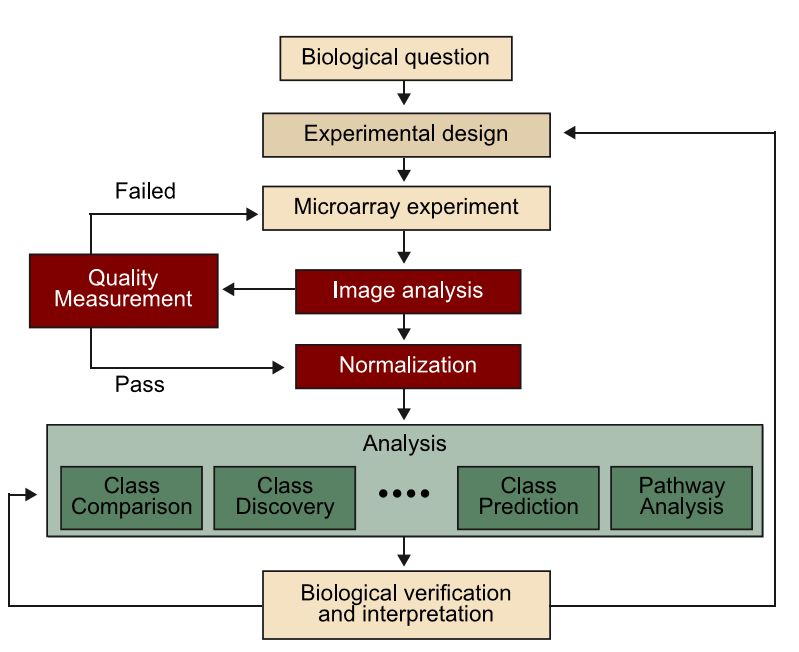
\includegraphics[width=0.9\textwidth]{Pipeline_Microarray.jpg} 
\caption{El procès d'anàlisi de microarrays}
\end{figure}

El \textit{pipeline} de l'anàlisi consisteix doncs en plantejament d'una pregunta i un disseny experimental a partir del qual és fa l'experiment de \textit{microarrays}. El producte d'experiment són bàsicament les images d'intensitats que es tradueixen als valors numèrics. Habitualment aquests valors són encara \textit{raw values} i han de ser processats adequadament. Aquest processament inclou el control de qualitat d'imatges i la normalització dels valors d'intensitat per reduir la variabilitat tècnica. Finalment les dades normalitzades s'utilitzen per a l'anàlisi estadístic. Habitualment la mesura natural per comparar les mostres és el \textit{log ratio} el qual podem denomiar alternativament \textit{logFC} on \textit{FC} es refereix a \textit{fold change}. Hi ha diversos tests estadístics per comprobal les difrències entre les mostres. En el cas de l'array d'un color podem fer servir tan els metodes paramètrics com ara el test T o mètodes del modelatge lineal o bé mètodes nonparamètrics com ara la proba de Mann-Whitney. El test adequat dependrà bàsicament de la distribució de les dades. El resultat d'aquest anàlisi serveix com a base per a interpretació biològica dels resultats d'experiment. Per poder fer sentit de les dades d'expressió i de l'anàlisi estadístic al nivell de gens és imprescindible fer un anàlisi a nivell de les categories de gens o les rutes. Per aquest anàlisi es necessita, com ho veurem a l'apartat següent, una llista ordenada de les expressions relatives (\textit{logFC}) i una subllista de gens que hem identificat mitjançant els tests estadístics com a diferencialment expressats.

En aquest treball m'ocupo de l'últim pas d'experiment d'escrit, més especificament amb l'anàlisi de rutes (\textit{Pathway analysis}).

La vista general de l'anàlisi de les rutes ofereix el gràfic següent:

\begin{figure}[H]
\centering
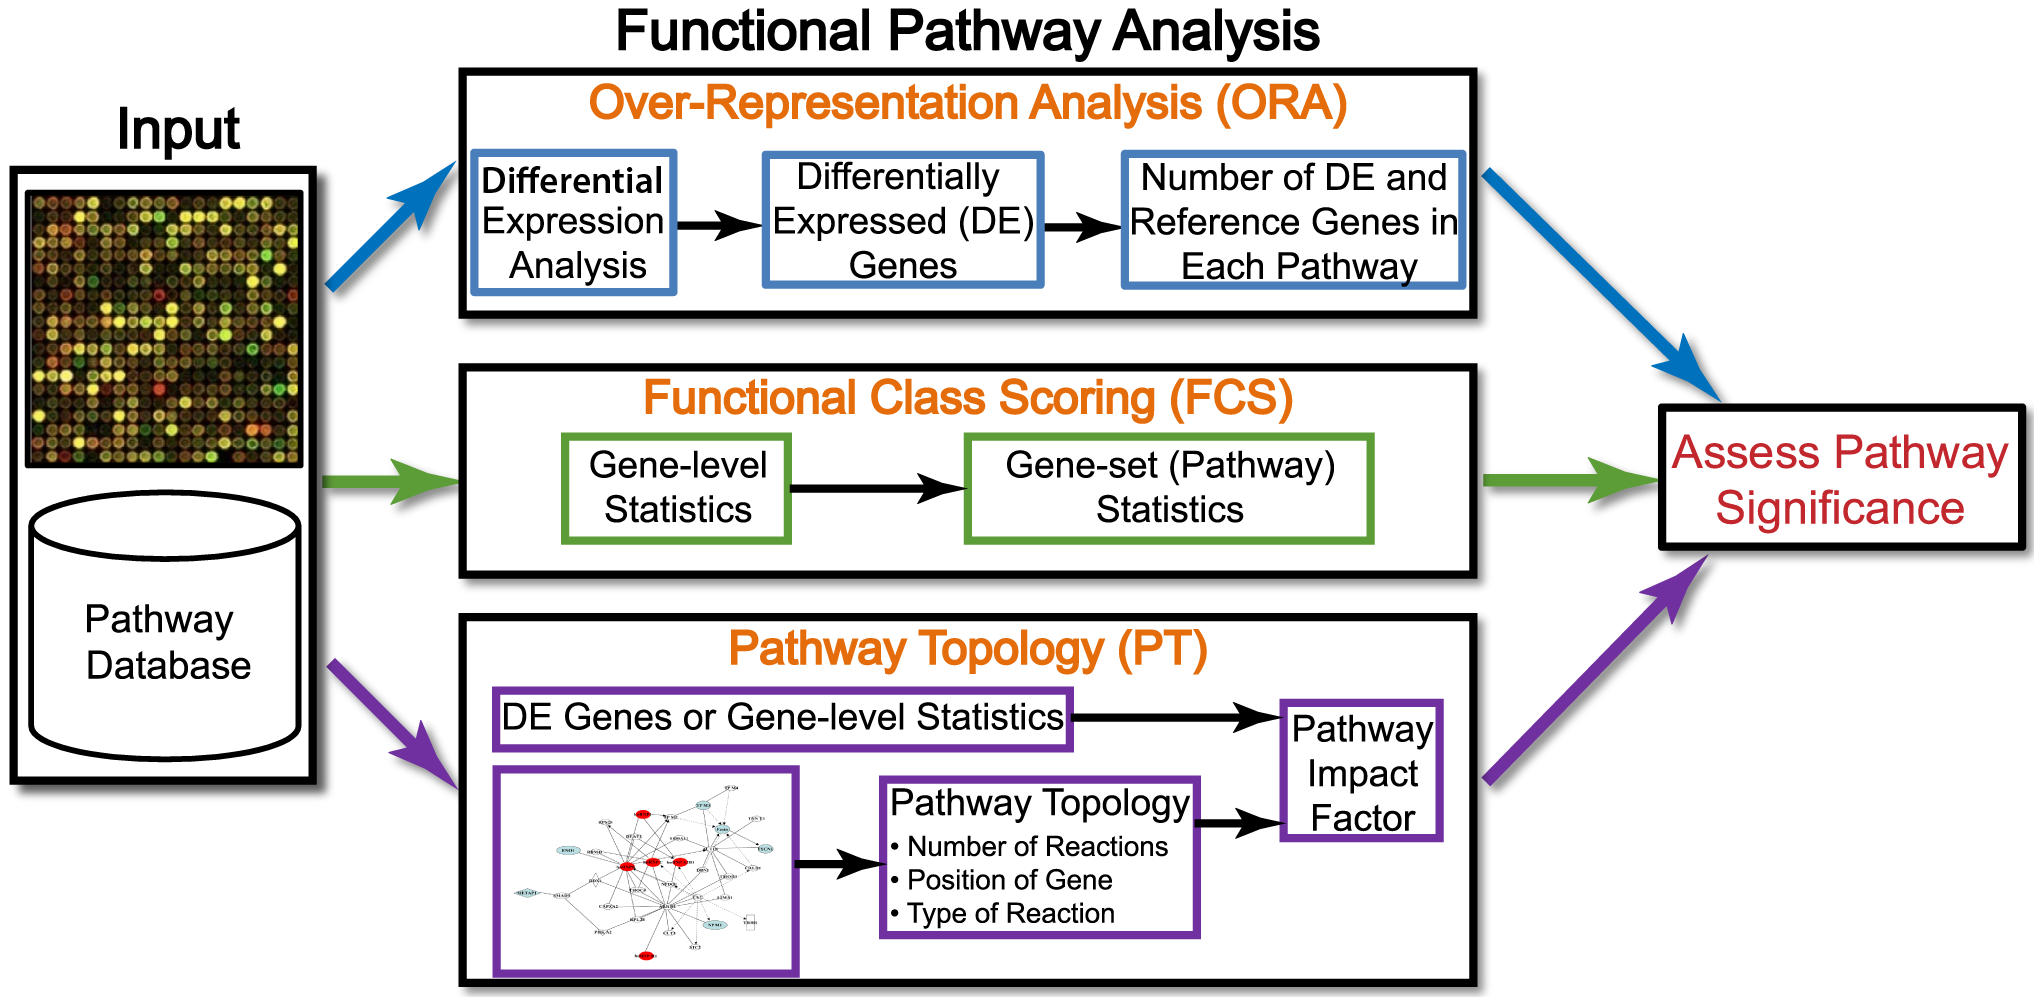
\includegraphics[width=0.9\textwidth]{Pipeline_Pathway.png} 
\caption{El procès d'anàlisi de les rutes}
\end{figure}

A part de les dades d'expressió, de les quals he parlat anteriorment, l'analisi requereix com a \textit{input} també la base de dades de les rutes. De les dades que utilitzaré a la meva aplicació en parlaré a la secció següent. Per ara hes important entendre que els resultats d'expressió s'anoten a les bases de dades existents per comprobar si els gens sobre o sotaexpressats pertanyen a unes rutes específica. Per comprobar aquesta, o millor dit, aquestes hipòtesis (per que hi hauran hipòtesis múltiples) s'han establert tres grups dels mètodes:

\begin{itemize}
\item \textbf{Over-Representation Anaysis (ORA)}.
Aquest anàlisi necessita la preselcció dels gens diferencialment expressats (DE) i copara la freqüència dels gens de la ruta d'interès en la mostra dels gens diferencialment expessats i la freqüencia dels gens de la ruta a la distrinució de fons. 
\item \textbf{Functional Class Scoring (FCS)}
Per a aquesta anàlisi no necessitem cap preselecció dels gens diferencialment expressats (DE) sinó ja basta amb tenir les estadístiques a nivell de gens, que al cas de l'aplicació és el \textit{logFC}.
\item \textbf{Pathway Topology (PT)}.
Aquest mètode enfoca la posició de gens diferèncialment expressats en la ruta i d'aquesta manera utilitza el coneixement de les bases de dades més àmplicament. Per exemple, si una ruta està activada per un sol producte genètic o mitjançant un reseptor i si aquesta proteïna particular no està produïda, la ruta estarà molt afectada, o fins i tot apagada. Més especifivacment, si el receptor d'insulina no és en la ruta d'insulina (\url{https://www.genome.jp/dbget-bin/www_bget?hsa04910}) tota la ruta serà desactivada (\cite{tarca2008novel}). D'altra banda si un nombre de gens està involucrar en la ruta però apareixen riu abaux el seu efecte podria ser menys important. A més a més també el nombre de coneccions amb altres gens a la ruta podria ser important \cite{rahnenfuhrer2004calculating}. O fins i tot leas estadístiques que incorporen factors diferents com ara la posició, el tipo d'interacció etc. \cite{draghici2007systems}.  Aquesta idea l'he implementat en l'aplicació afegint les rutes dibuixades de KEGG i Reactome, on els gens estan emfatitzats d'acord amb els \textit{logFCs} obtinguts mitjançant l'experiment.


\end{itemize}

Els mètodes interessants per a dur a terme l'anàlisi de les rutes són:

\begin{itemize}
\item ORA \cite{boyle2004go}
\item Mètodes GSA
\begin{itemize} 
\item Permutació de les mostres: GSEA \cite{subramanian2005gene}, SAFE \cite{dinu2007improving} com els més representatius;
\item Permutació dels gens: PAGE \cite{kim2005page}, T-Profiler \cite{newton2007random} com els més representatius.
\end{itemize}
\item GAGE (Generally Applicable Gene set Enrichment for pathway analysis) \cite{luo2009gage}
\end{itemize}

Per fer l'aplicació més estructurada i menys complicada he elegit al final els dos mètodes: ORA \cite{boyle2004go} i GSEA \cite{subramanian2005gene}. L'anàlisi GAGE seria un bon \textit{Add-on} però per falta de temps per completar el TFM al final he decidit concentrar-me exclusivament en ORA i GSEA , els mètodes que descriure a les seccions següents.

\subsection{Annotació dels gens}

Com veurem més endavant per a anàlisi de les rutes és imprescindible tenir com a referència anotacions dels gens. Per a aplicació he utilitzat tres bases de dades: Gene Onthology (GO), Kyoto Encyclopedia of Genes and Genomes i Reactome. 

\subsubsection{Gene ontology}
Gene Ontology \cite{gene2004gene} dona tan un vocabulari estructurat i controlat (ontologies) com la classificació que cobreix alguns dominis de la biologia molecular i cel·lular. És una base de dades gratuïta per a anotació de gens, el seu producte i les seqüències. El projecte GO proporciona ontologies per a descriure els atributs dels productes de gens als tres dominis separats de la biologia molecular:
\begin{enumerate}
\item \textbf{Molecular Function (MF)}. Aquest domini descriu activitats al nivel·l molecular. És important entendré que el terme ``molecular function'' representa més les activitats i no pas les entitats (com per exemple molecules o complexos) que fan aquestes accions i a més a més no espeifíquen quan o a quin context l'acció té lloc. Un exemple podria ser \textit{catalytic activity} o un terme més específic \textit{adenylate cyclase activity}.
\item \textbf{Biological Process (BP)}. Aquest domini descriu els objectius biològics aconseguits per una o conjunt de les funcions moleculars. Un exemple d'un procès biològic ampli podria se \textit{DNA repair}. Un exemple més específic podria se \textit{pyrimidine nucleobase biosynthetic process}. 
\item \textbf{Cellular Component (CC)}. EL CC descriu l'emplaçaments al nivell d'estructures subcel·lulars (com \textit{mitocondri}) i els complexos macromoleculars (com \textit{ribisomes}) on el producte de gen fa la seva funció.
\end{enumerate}

Dins de cada ontologia, els termens tenen tan una definició de text com un identificador únic. El vocabulari està estructurat en una classificació que manté les relacions ``is-a'' i ``part-of'' i ``regulates''. Aquestes relacions les descriu amb més detall més endavant en la secció dedicada al gràfic acíclic de GO termes.

\subsubsection{KEGG}
La base de dades KEGG és la col·lecció del mapes dibuixades manualment que representen el coneixemnet sobre interacció molecular dividit eb set dominis principals:
\begin{enumerate}
\item Metabolism
\item Genetic Information Processing
\item Environmental Information Processing
\item Cellular Processes
\item Organismal Systems
\item Human Deseases
\item Drug Development
\end{enumerate}

Els mapes són dibuixades amb un software específi (KegSketch) que genera un arciu KGML+. Aquest arxiu és un arxiu SVG que conté els objectes gràfics que són associats amb els objectes KEGG. Els objectes gràfics bàsics de les rutes KEGG són:
\begin{itemize}
\item caixes: gens o el seu producte
\item cercles: altres molècules
\item línies: reaccions
\end{itemize}
 
El significat més detallat d'aquests elements el presentaré a la secció dedicada a les rutes KEGG.

\subsubsection{Reactome}

Reactome és una base de dades gratuitament accecible i manualment curada per a reaccions i rutes biològiques. Al centre de Reactome són reaccions que es definexen com qualsevol esdeveniment molecular com ara unió, fosforilització, catàlisi bioquèmic, transport molecular o esdeveniments moleculars espontani. Aquestes reaccions involucren qualsevol molècula, però més típicament passen entre proteïnes i les molècules petites. Encara que els mapes de Reactome disponibles online contenen una relació entre les molecules més detallada el paquete de Bioconductor que utilitzaré per generar els mapes visualitza només la conecció bàsica entre els gens. 

\subsection{ORA}

L'anàlisi de sobreexpressió és una tècnica d'identificació de les rutes significativament enriquides en la mostra d'interès. 

El paper original que se cita habitualment quan es parla d'anàlisi d'expressió genètica és de \cite{boyle2004go}. El mètode estadístic descrit consisteix bàsicament en els passos següents:

\begin{enumerate}
\item \textbf{De tots els gens de la mostra seleccionar un grup de gens que es considera que són significativament expressats.}

Els criteris de selecció poden basar-se en \textit{log ratios} i/o en el valor de p provinent d'un test estadístic. \textit{Log ratios} donen la magnitud amb la qual un gen és sobre o sotaexpressat. Les diferències entre els grups però són el resultat d'un procès estochàstic i per tant hem d'intentar de minimitzar el risc de prendre decisions falses. El valor de p representa la probabilitat d'aquest risc i per tant dona certa confiança sobre la significació de les diferències observades.

\item \textbf{Determinar si algunes rutes anoten la llista especificada de gens amb la freqüència més alta que la que s’esperaria per casualitat.} 

El test estadístic es basa en la distribució hipergeomètrica: 

$$p = 1 - \displaystyle\sum_{i = 0}^{k-1}\frac{{M \choose i}{{N-M} \choose {n-i}}} {{N \choose n}}$$

En aquesta equació $N$ és el nombre total de gens en la distribució de fons, $M$ és el nombre de gens dins d'aquesta distribució que són anotats a la ruta d'interès, $n$ és el nombre total en la llista especificada de gens i $k$ és el nombre de gens dins d'aquesta llista que són anotats a la ruta. La distribució de fons pot ser o bé tots els gens en la base de dades d'anotació o bé tots els gens de l'experiment.

El valor de P obtingut amb aquesta fòrmula dona la probabilitat de veure el nombre $x$ de gens de la llista relacionats amb la ruta específica en la llista del nombre total de gens $n$ donat la proporció de gens relacionats amb aquesta ruta en la distibucó de fons.
\end{enumerate}

L'aplicació utilitza aquesta idea i calcula una taula amb els camps següents:


\begin{itemize}
\item \underline{Description}. El nom del terme GO;
\item \underline{GeneRatio}. El quocient: $\displaystyle\frac{\mbox{Nombre dels gens diferencialment expressats que pertanyen al conjunt de gens}}{\mbox{Nombre total dels gens diferencialment expressats}}=\frac{M}{N}$; 
\item \underline{BgRatio}. El quocient: $\displaystyle\frac{\mbox{Nombre dels gens del conjunt d'interès en la distribució de fons}}{\mbox{Nombre total dels gens en la distribució de fons}}=\frac{k}{n}$;
\item \underline{pvalue}. Valor de p basat en la distribució hipergeomètrica descrita anteriorment.
\item \underline{p.adjust}. El valor de P ajustat. L'usuari pot seleccionar el mètode d'ajustmanent.
\end{itemize}


\subsection{GSEA}

Amb l'anàlisi GSEA podem analitzar els resultats d'un experiment d'expressió per a dos grups. Aquí els gens són ordenats basant-se en la correlació entre la seva expressió i la separació entre les classes. Aquest llistat ordenat $L$ el podem crear utilitzant els \textit{logRatios}.

Donat el conjunt definit dels gens $S$, que pertanyen per exemple al mateix terme de Gene Ontology, l'objectiu de GSEA és determinar si els membres de $S$ són distribuïts aleatòriament en el $L$ o es troben més al cap o a la cua. S'esperaria que els gens relacionats amb la separació fenotípica mostraran aquesta última distribució. 

L'anàlisi GSEA consisteix en tres passos:

\begin{enumerate}
\item Càlcul de la puntuació d'enriquement (\textit{ES: Enrichment Score}). La puntuació està calculada anant per la llista i augmentant la suma corrent sempre quan es troba un gen que pertany a $S$ o, al contrari, restant-la quan el gen no forma part del conjunt $S$. La puntuació és la desviació màxima del zero observada en aquet camí. L'estadística obtinguda és l’estadística de Kolmogorov-Smirnov amb pesos.

\item Estimació del nivell de significació per a la puntuació \textit{ES}. El valor de P nominal es pot obtenir mitjançant o bé la permutació de les classes o bé la permutació de gens, on l'estadística \textit{ES} observada es compara amb la distribució obtinguda amb permutació. A l'aplicació es fa ús de l'útima opció.
\item Càlcul del valor de P ajustat. El valor de P nominal s'ajusta per controlar l'error global que es produeix com a resultat de les comparacions múltiples.
\end{enumerate}

\begin{figure}[H]
\centering
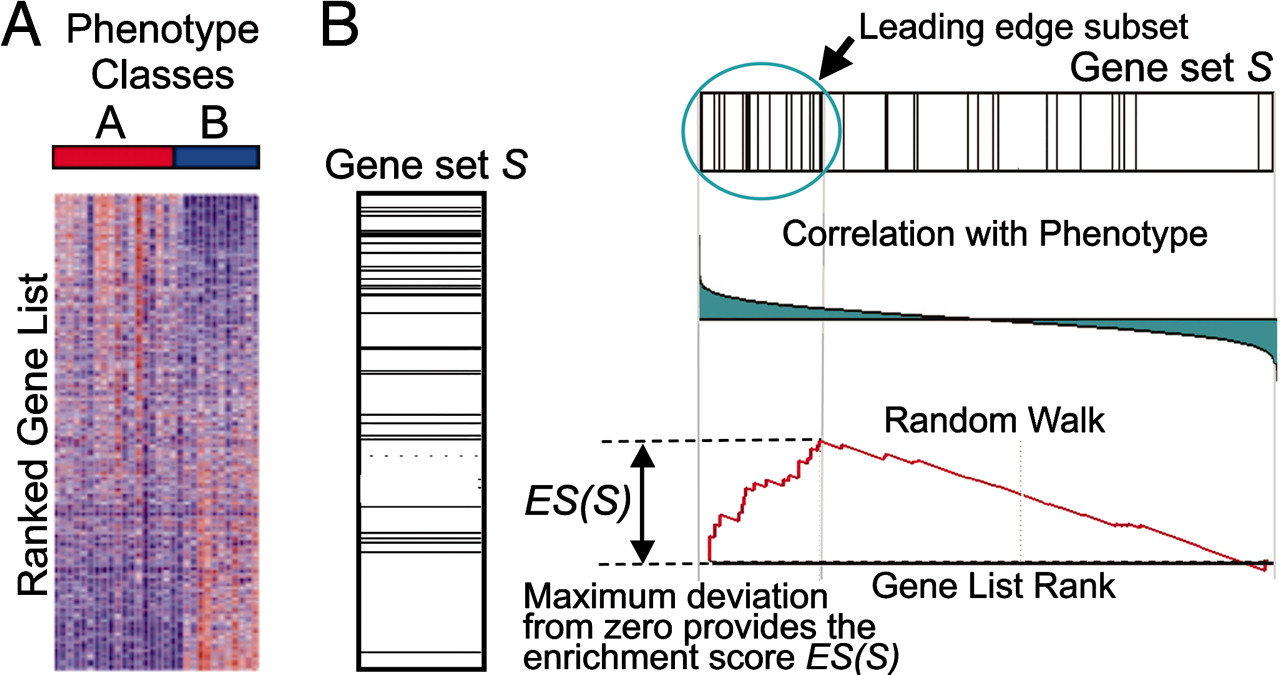
\includegraphics[width=0.9\textwidth]{GSEA_Method.jpg} 
\caption{El mètode GSEA}
\end{figure}

L'aplicació que he desenvolupat agafa aquesta idea i calcula la taula que inclou les estadístiques següents:

\begin{itemize}
\item \underline{enrichmentScore}. Enrichment score per al conjunt dels gens. Amb altres paraules: el grau amb el qual el conjunt dels gens està sobreexpressat a dalt o a baix del llistat ordenat dels gens en les dades d'expressió.
\item \underline{NES}. Normalized enrichment score. La puntuació per al conjunt de gens després de ser normalitzat tenint en compte tots els conjunts de gens analitzats (la seva mida i la seva correlació amb les dades d'expressió). Aquesta puntuació ajuda a comparar els resultats entre els conjunts de gens.
\item \underline{pvalue}.El valor de p nominal.
\item \underline{p.adjust}. El valor de p ajustat.
\item \underline{leading\_edge}
\begin{itemize}
\item \underline{Tags}. El percentatge de les ocurrències de gens del conjunt específic abans (per als ES positius) o després (per als ES negatius) del cim en la puntuació corrent d'enriquiment. Aquest valor indica el percentatge dels gens que contribueixen a la puntuació d'enriquement. 
\item \underline{List}. El percentatge dels gens en el llistat ordenat de tots els gens abans o després del pic en la puntuació corrent d'enriquiment. Aquest valor ens indica on exactament el pic es produeix. 
\item \underline{Signal}. La fortalesa del senyal d'enriquiment que combina els dos valors anteriors.
\end{itemize}
\item \underline{rank}. La posició del pic en la llista ordenada dels gens. Els conjunts dels gens més interessants assoleixen el seu màxim o bé al principi o al final de la llista ordenada. Vol dir que tenen aquest valor o bé molt baix o bé molt alt.
\end{itemize}

\subsection{L'anàlisi topològic de les rutes}
Tan ORA com GSEA no visualitzen les relacions entre les rutes i entre els gens dins de les rutes. Els avenços en anotació manual de les bases de dades disponibles (GO, KEGG i Reactome) contenen però aquesta informació i l'aplicació, gràcies al paquet \helvetica{clusterProfiler}, hi treu l'avantatge i visualitza aquestes relacions més detalladament. 

\subsubsection{El mapa d'enriquement}

Navegant a la categoria \textbf{Enrichment plot} l'usuari obté el mapa d'enriqument. El mapa organitza les rutes en una xarxa amb les línies que connecten les rutes amb els gens solpats. D'aquesta manera les rutes amb gens en comú s'agrupen més a prop l'una de l'altra.

\subsubsection{Gene-Concept-Network}

L'anàlisi ORA no visualitza per si sola els gens que contribueixen al fet que la ruta sigui diferencialment expressada. Amb la xarxa de gens-concepte es pretén visualitzar els gens al voltant dels conceptes on els gens poden ser connectats amb les rutes (conceptes) diferents. D'aquesta manera es fa possible identificar les associasions biològiques més complexes entre les rutes mitjançant els gens. 

\subsubsection{GOplot}
%Per a mès informació http://geneontology.org/docs/ontology-relations/

El gràfic de GO està organitzat com direccional acíclic gràfic (Directed Acyclic Graph). Una manera útil de veure els resultats és mirar com els termes GO estan distribuïts per aquest gràfic. L'aplicació ensenya el gràfic GO induït pels els gens més significatius. El gràfic mostra tres relacions possibles entre les rutes: 
\begin{enumerate}
\item \textit{is a}: Si dèiem que A \textit{is a} B, volem dir que A és un subtip de B. Per exemple el cicle mitòtic de la cèl·lula \textit{is a} cicle de la cèl·lula. 
\item \textit{part of}: Aquesta relació s'utilitza per representar la relació entre una part i el tot. Aquesta relació entre A i B existeix nomès si B és necessàriament una part d'A: quan B existeix, ho fa només com una part de B i la presència de B implica la presència d’A.
\item \textit{regulates}: La relació descriu el cas on un procès afecta directament la manifestació de l'altre procès.
\end{enumerate}

Els conceptes al llarg del gràfic són marcats amb color depenent si són estadísticament significatius o no.

\subsubsection{KEGG Pathway}
%Per a més informació sobre l'anotació https://www.genome.jp/kegg/document/help_pathway.html
Aquest gràfic mostra les relacións entre els gens dins de la ruta específica. Els gens són remarcats amb el color depenent de l'expressió diferencial mesurada amb LogRatios. Per poder interpretar el gràfic és útil tenir present l'anotació següent:

\begin{figure}[H]
\centering
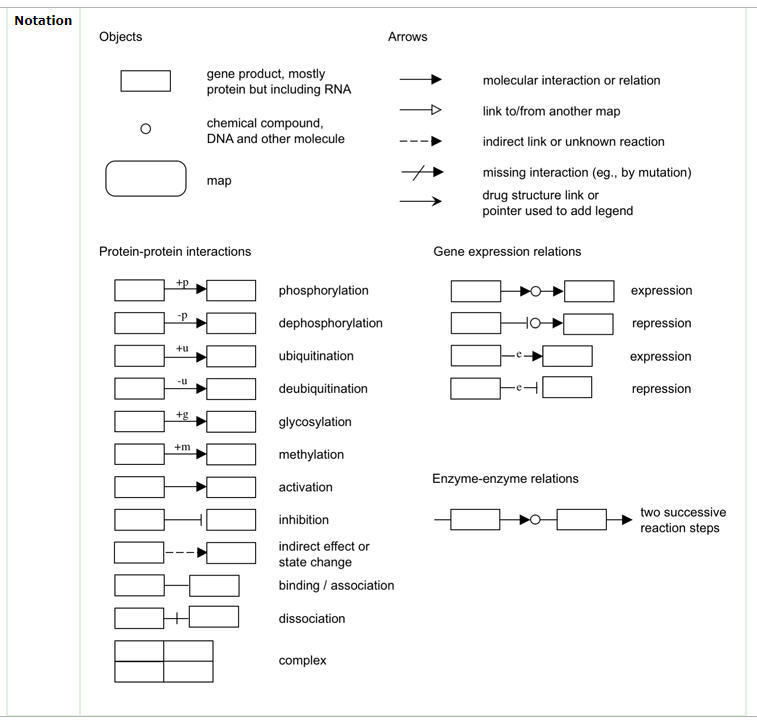
\includegraphics[width=0.9\textwidth]{Annotation_KEGG.jpg} 
\caption{L'anotació de les relacions dins de les rutes KEGG}
\end{figure}

\subsubsection{Reactome Pathway}
En canvi a Goplot i les rutes KEGG les relacions entre els gens dins les rutes Reactome són més senzilles. Aquí les relacions són mostrades només amb les línies, on es pot interpretar només la distància entre els gens. 

\section{Tractament bioinformàtic}

\subsection{Cerca dels paquets de Bioconductor}

El paquet \helvetica{clusterProfiler} de Bioconductor integra els mètodes per dur a terme l'anàlisi de les rutes basant-se en les bases de dades GO, KEGG i Reactome. Els dos mètodes principals són ORA (Overrepresentation analysis) i GSEA (Gene set enrichment Analysis). També inclou les possibilitats de visualització dels resultats suficients per considerar l'anàlisi de les rutes complet. Notem però que el test de permutació a l'anàlisi GSEA implementat per clusterPrifiler es basa en la permutació dels gens i no de les mostres com originalment és proposat per \cite{subramanian2005gene}.

\subsection{Desenvolupar el protocol}

Crec que l'aplicació és molt intuitiva i deixa entreveure l'esquema següent:

\begin{figure}[H]
\centering
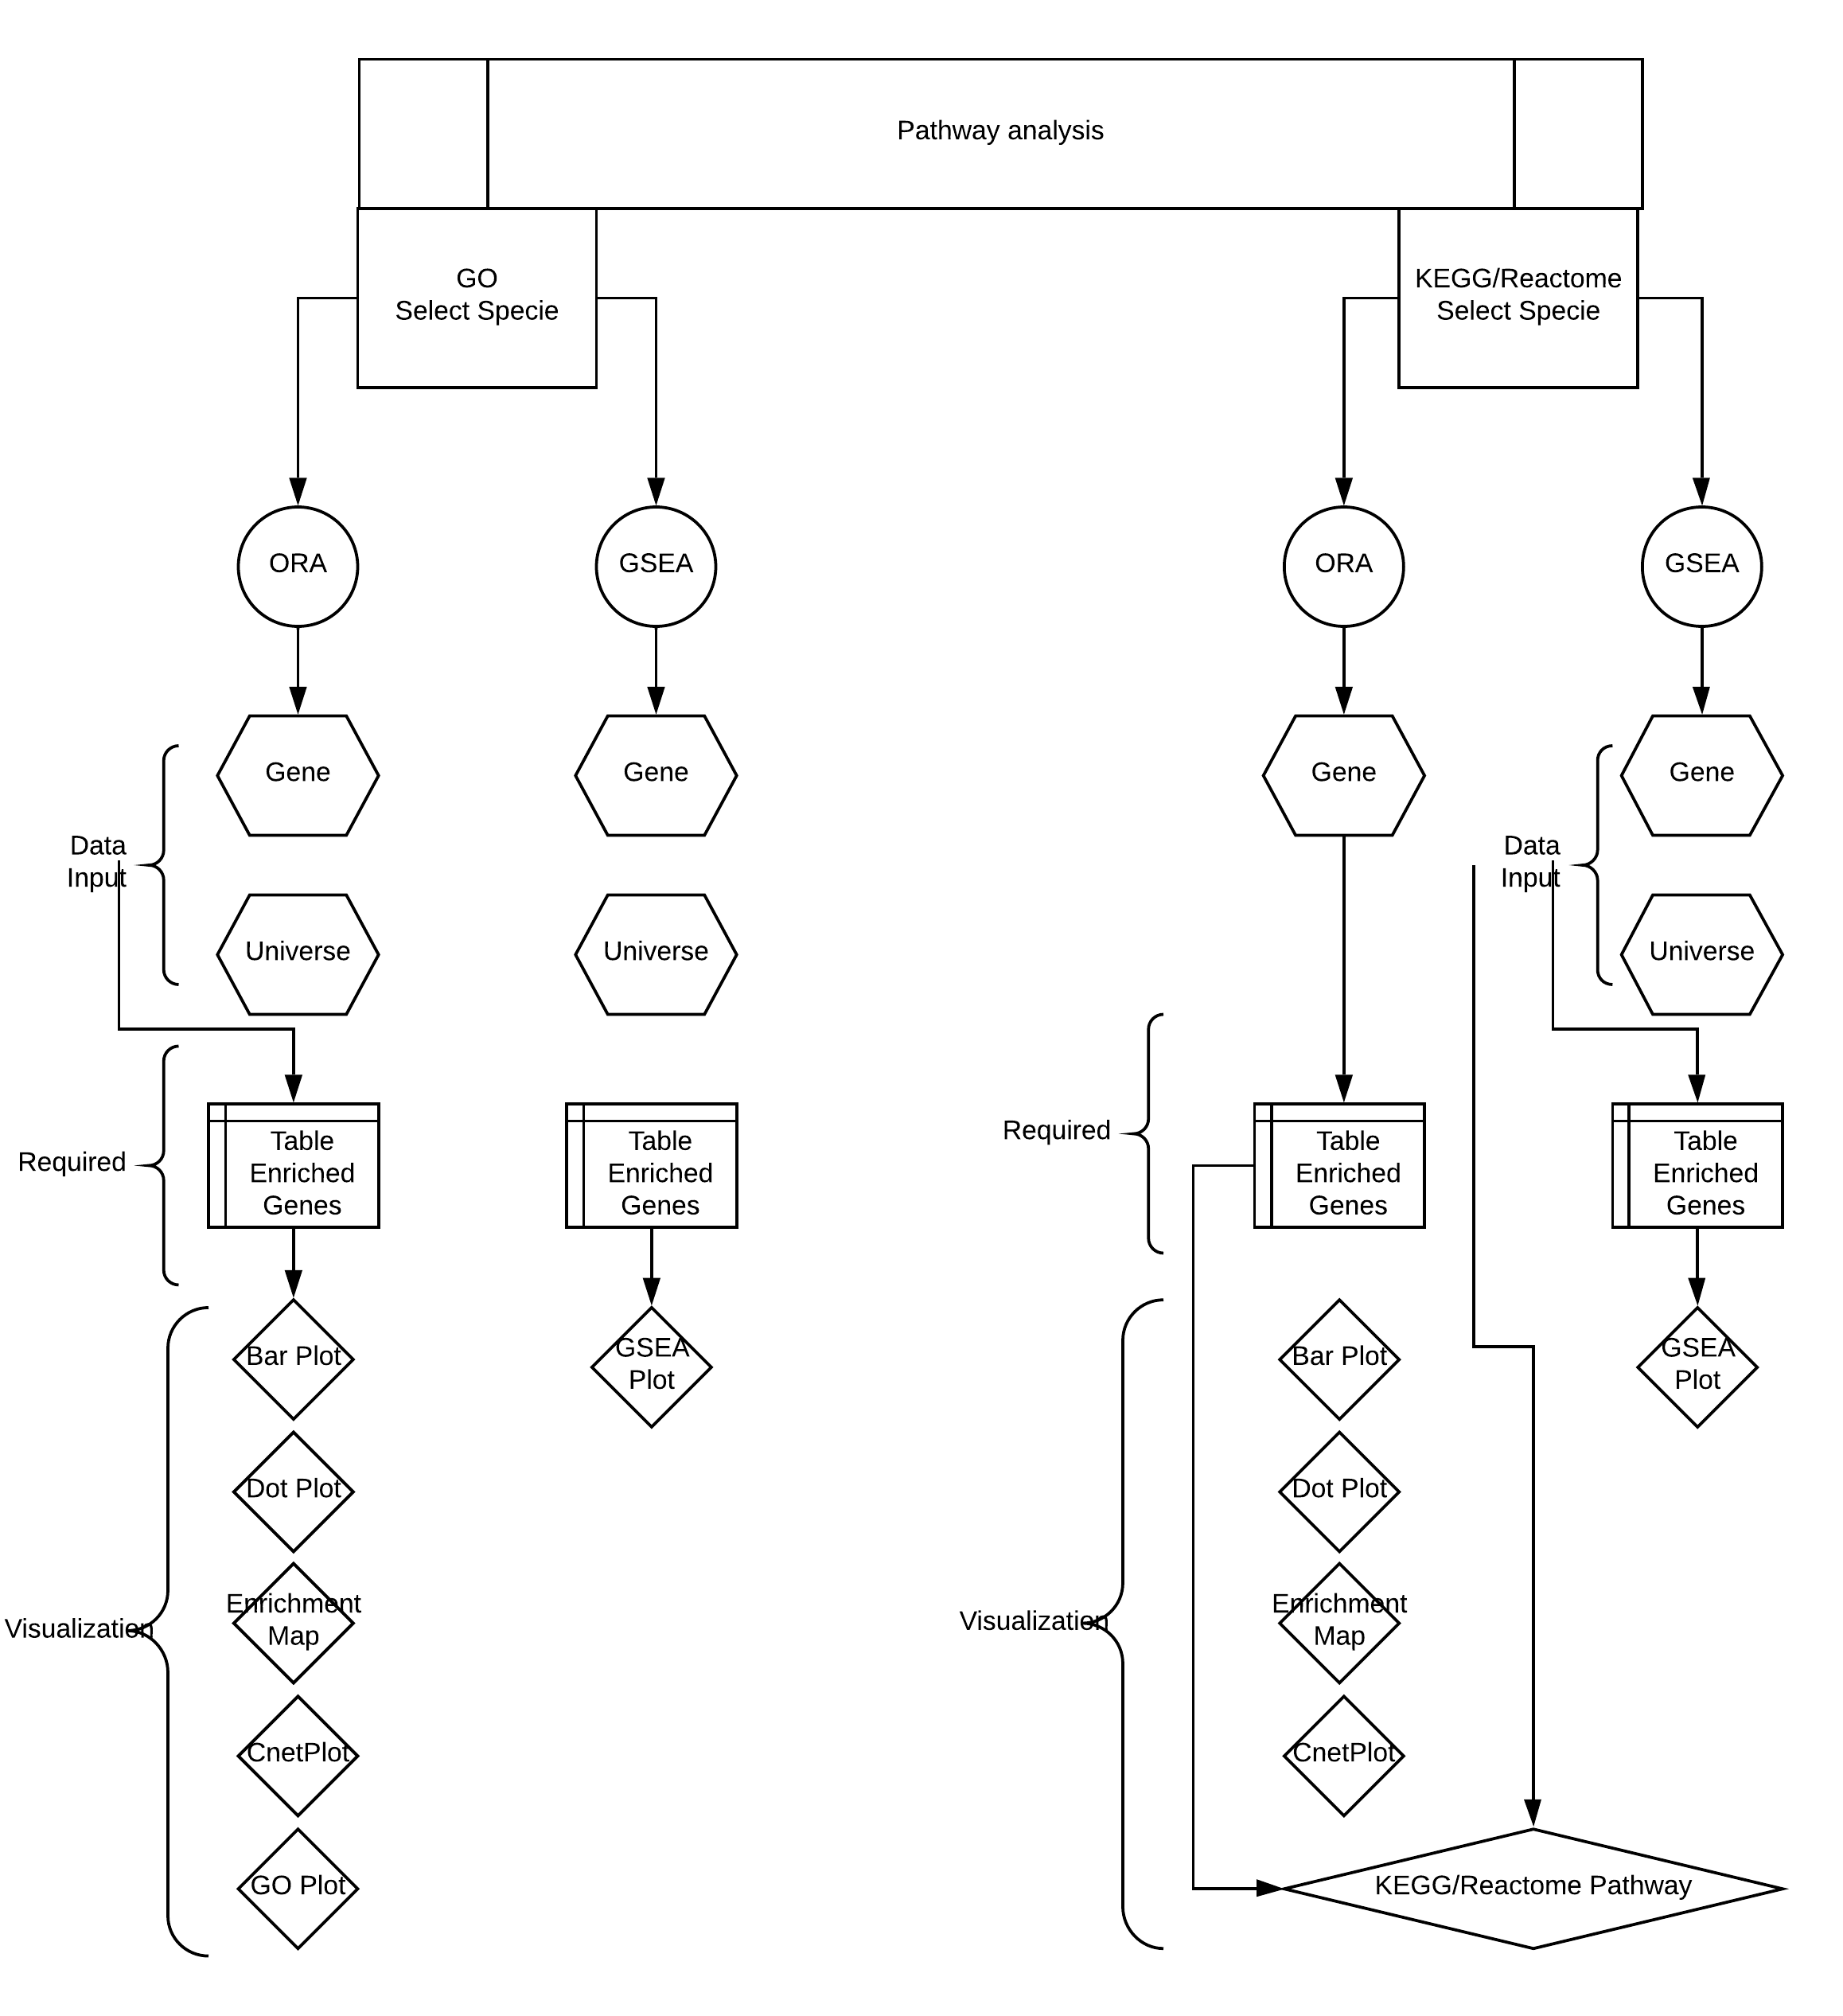
\includegraphics[width=0.9\textwidth]{LucidChart.png} 
\caption{Lucidchart per a l'aplicació}
\end{figure}

D'aquí podem definir per exemple el protocol:
\begin{enumerate}
\item Decidir quin anàlisi vol fer: GO, KEGG o Reactome
\item Seleccionar l'espècie de referència
\item Decidir quin mètode vol implementar: ORA o GSEA i respectivament pujar les dades necessàries.

$\rightarrow$ Per a anàlisi GO tots dos arxius són necessaris: Gens Seleccionats (Gene) i Tots els gens (Universe). 

$\rightarrow$ Per a l'anàlisi KEGG o Reactome les dades necessàries varien: Pel mètode ORA l'arxiu amb els gens seleccionats és suficient. Dos arxius són necessaris pel mètode GSEA.
\item En el cas que volguem fer l'anàlisis ORA seleccionar a l'apartat corresponent (GO, KEGG o Reactome) la pestanya ORA i definir els criteris.

$\rightarrow$ Els gràfics: Bar Plot, Dot Plot Enrichment Map, Cnet Plot, GO Plot (en cas d'anàlisi GO) i els gràfics de les rutes (KEGG/Reactome) es calculen automàticament

\item En el cas que volguem fer l'anàlisi GSEA seleccionar a l'apartat corresponent (GO, KEGG o Reactome) la pestanya GSEA i definir els criteris.

$\rightarrow$ El gràfic GSEA es genera automàticament. Es pot elegir la ruta mitjançant un menú desplegable.

\end{enumerate}


\section{Instal·lació de l'aplicació}

La solució més plausible i ràpida era empaquetar tota l'aplicació dins d'un paquet R i fer-la disponible d'aquesta manera en el GitHub. Hi havia també dues opcións més: 

\begin{itemize}
\item Publicar l'aplicació a CRAN
\item Publicar l'aplicació en un servidor Shiny
\end{itemize}
La primera opció, publicació en CRAN, no l’he contemplat encara, perquè la solució no és immediata, sino que és un procès que no és fàcil i pot tardar fins que el paquet estigui
 publicat amb éxit. Com comenta \cite{HWick} \enquote{submitting to CRAN is a lot more work than just providing a version on github, but the vast majority of R users do not install packages from github, because CRAN provides discoverability, ease of installation and a stamp of authenticity. The CRAN submission process can be frustrating, but it’s worthwhile...}. Normalment els paquets han d’estar en perfectes condicions abans d'entregar-los i seran revisats manualmet per un equip dels voluntaris. D'aquesta manera l'aplicació no seria avaluable dins del marc temporal previst per al treball de màster. A més a més considero que podria millorar encara més l'aplicació abans d'entregar-lo.

La segona opció, publicació via Shiny Server, és molt interessant, però implicaria un treball considerable per configurar el servidor. Com que ho faria per primera vegada, no puc assegurar que tot estigui preparat a temps. 

Per tant, el paquet \helvetica{PathwayApp} es pot instal•lar del repositori GitHub seguint els passos següents:

\begin{enumerate}
\item Instal·lar, si encara no està fet, la versió actual de R;

\item Instal·lar, si encara no està fet, el Bioconductor;

\item Instal·lar, si encara no està fet, el paquet \helvetica{devtools}

\begin{lstlisting}[language=R]
install.packages(``devtools'')
library(devtools)
\end{lstlisting}

\item Instal·lar el paquet \helvetica{PathwayApp}

\begin{lstlisting}[language=R]
devtools::install_github("vdruchkiv/TFM/5_Packages/PathwayApp/PathwayApp")
\end{lstlisting}

\item Iniciar l'aplicació 
\begin{lstlisting}[language=R]
PathwayApp::runPathwayApp()
\end{lstlisting}
\end{enumerate}

La funció \helvetica{runPathwayApp()} iniciarà la comprovació dels paquets necessaris i començarà l'aplicació. Els paquets següents seran instal·lats, si no ho són encara:

\begin{center}
\begin{tabular}{||c | c ||} 
\hline\hline 
\textbf{Paquet} & \textbf{Font} \\ [0.5ex] 
\hline\hline
clusterProfiler & Bioconductor \\
\hline
ReactomePA & Bioconductor \\
\hline
pathview & Bioconductor \\ 
\hline
pathviewPatched & GitHub vdruchkiv/TFM\\
\hline
dplyr & CRAN \\
\hline 
ggplot2 & CRAN \\
\hline
knitr & CRAN \\
\hline
kableExtra & CRAN \\
\hline
formattable & CRAN \\
\hline
shiny & CRAN \\
\hline 
shinydashboard & CRAN \\ 
\hline
shinyhelper & CRAN \\
\hline 
shinycssloaders & CRAN\\
\hline\hline
\end{tabular}
\end{center}


\section{L'anàlisi comuna de GO, KEGG i Reactome}
\label{sec:ACom}

\subsection{ORA}

\subsubsection{GO}

Per realitzar l'anàlisi ORA per a termes GO s'utilitza la funció \helvetica{enrichGO} del paquet \helvetica{clusterPrifiler}.
\begin{lstlisting}[language=R]
enrichGO(gene, OrgDb, keyType = "ENTREZID", ont = "MF", pvalueCutoff = 0.05, 
pAdjustMethod = "BH", universe, qvalueCutoff = 0.2, minGSSize = 10, maxGSSize = 500, 
readable = FALSE, pool = FALSE)
\end{lstlisting}

He implementat els valors per defecte amb la possibilitat per a l’usuari d'elegir entre:

\begin{itemize}
\item \underline{Ontologies GO} 
\begin{itemize}
\item Molecular function, Biological proces, Cellular Components;
\end{itemize}
\item \underline{Nivell de significació basant-se en els valors de P ajustats}
\begin{itemize}
\item 0.1, 0.05, 0.01, 0.001;
\end{itemize}
\item \underline{Mètode d'ajustament}
\begin{itemize}
\item Holm; Hochberg; Hommel; Bonferroni; BH; BY; FDR; None.
\end{itemize}
\end{itemize}

\begin{figure}[h!]
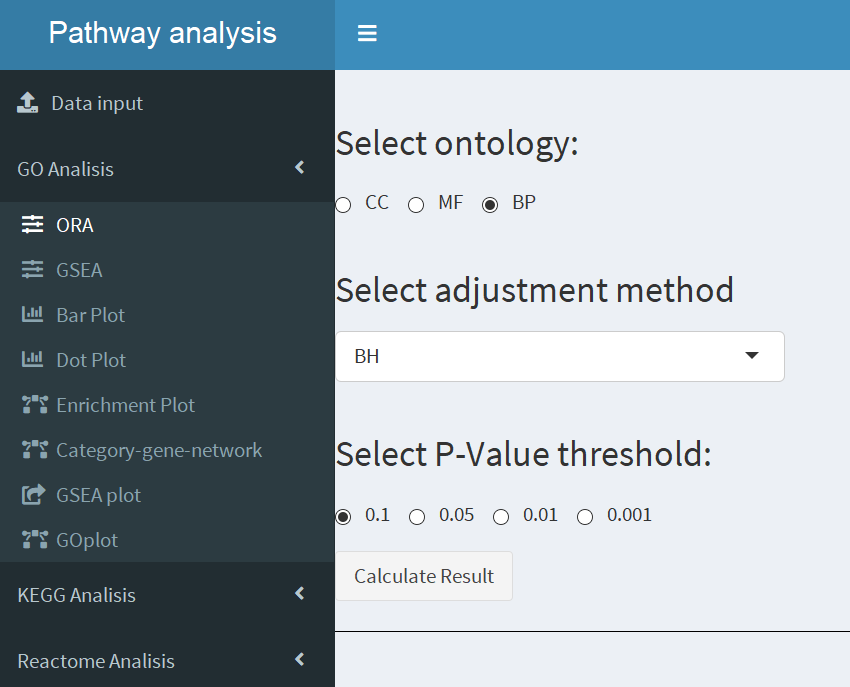
\includegraphics[width=0.9\textwidth]{App_F5_Items_GO_ORA.png}
\caption{Especificació d'ORA dels termes GO}
\end{figure}
L'execució de la funció és un procès temporalment costós. Per aquest motiu he afegit el botó d'acció, en lloc de deixar la funció reactiva. D'aquesta manera l'usuari ha de fer una decisió conscient de repetir l'anàlisi amb altres valors.

Prement el botó apareix la taula i el botó nou mitjançant el qual l'usuari pot descarregar els resultats en format .csv. He formatejat la taula amb els paquets \helvetica{knitr}, \helvetica{kableExtra}, \helvetica{formattable} i \helvetica{dplyr}. Amb els dos últims he afegit les barres de color pel nombre dels gens diferencialment expressats del terme específic de GO i la gradació de color del verd fins al vermell pels valors dels més petits fins els més grans. 

\begin{figure}[h!]
\centering
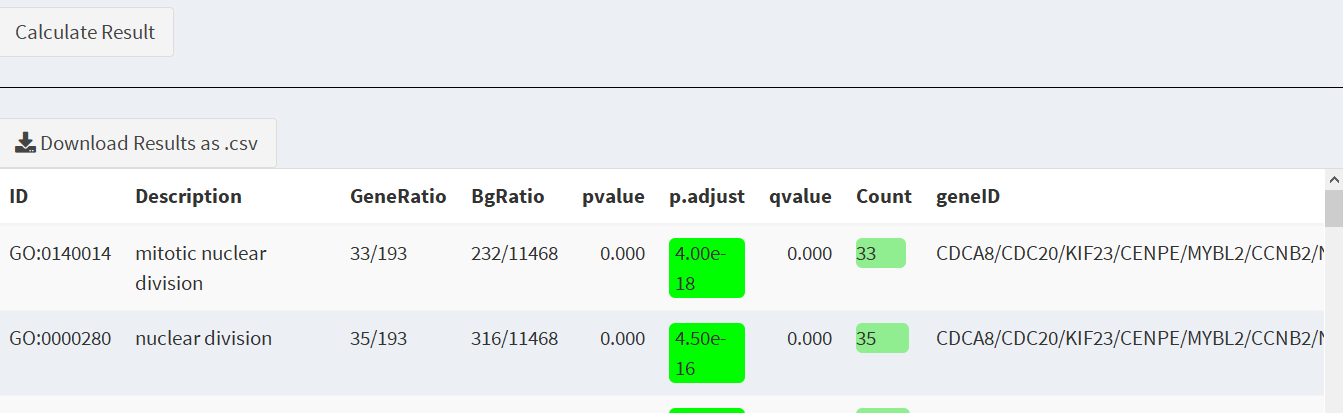
\includegraphics[width=0.9\textwidth]{App_F6_Items_GO_ORA_Table.png} 
\caption{El resultat d'anàlisi ORA. GO.}
\end{figure}


\subsubsection{KEGG}

Per l'ORA de base de dades KEGG he utilitzat la funció \helvetica{enrichKEGG()} del paquet \helvetica{clusterProfiler}. 

\begin{lstlisting}[language=R]
enrichKEGG(gene, organism = "hsa", keyType = "kegg", pvalueCutoff = 0.05, 
pAdjustMethod = "BH", universe, minGSSize = 10, maxGSSize = 500, 
qvalueCutoff = 0.2, use_internal_data = FALSE)
\end{lstlisting}



\begin{figure}[H]
\centering
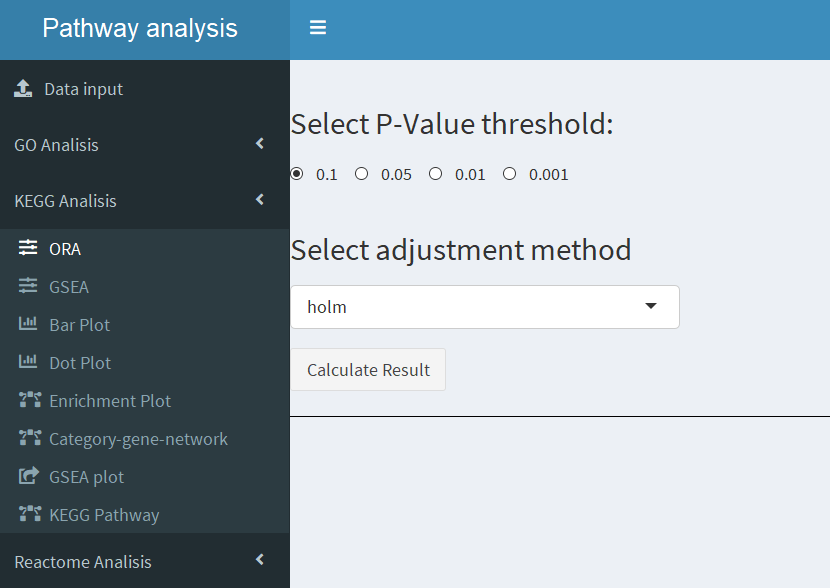
\includegraphics[width=0.9\textwidth]{App_F7_Items_KEGG_ORA.png} 
\caption{Configuració d'anàlisi KEGG}
\end{figure}



Una vegada introduïts els paràmetres i premut el botó \textbf{Calculate} apareix el botó \textbf{Download .csv} i la taula previsualitzada. Els camps de la taula són els mateixos com en l'anàlisi dels termes GO.
\begin{figure}[H]
\centering
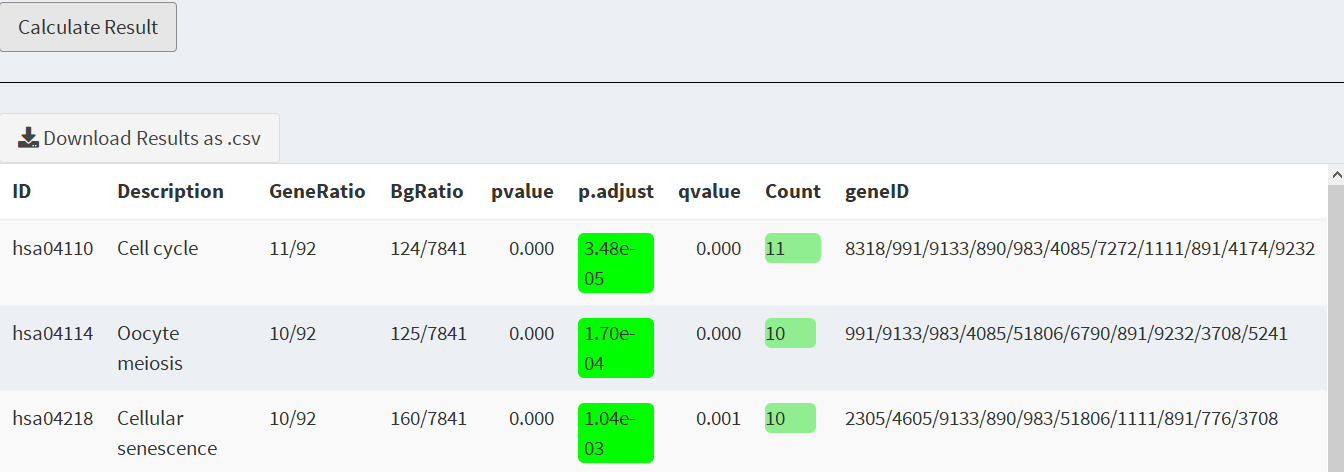
\includegraphics[width=0.9\textwidth]{App_F9_Items_KEGG_ORA_Table.png} 
\caption{El resultat de l'anàlisi ORA. KEGG.}
\end{figure}

\subsubsection{Reactome}
En el cas de Reactome el procediment és similar. La funció usada és \helvetica{enrichPathway()} del paquet \helvetica{ReactomePA}:

\begin{lstlisting}[language=R]
enrichPathway(gene, organism = "human", pvalueCutoff = 0.05,
pAdjustMethod = "BH", qvalueCutoff = 0.2, universe, minGSSize = 10,
maxGSSize = 500, readable = FALSE)
\end{lstlisting}


\begin{figure}[H]
\centering
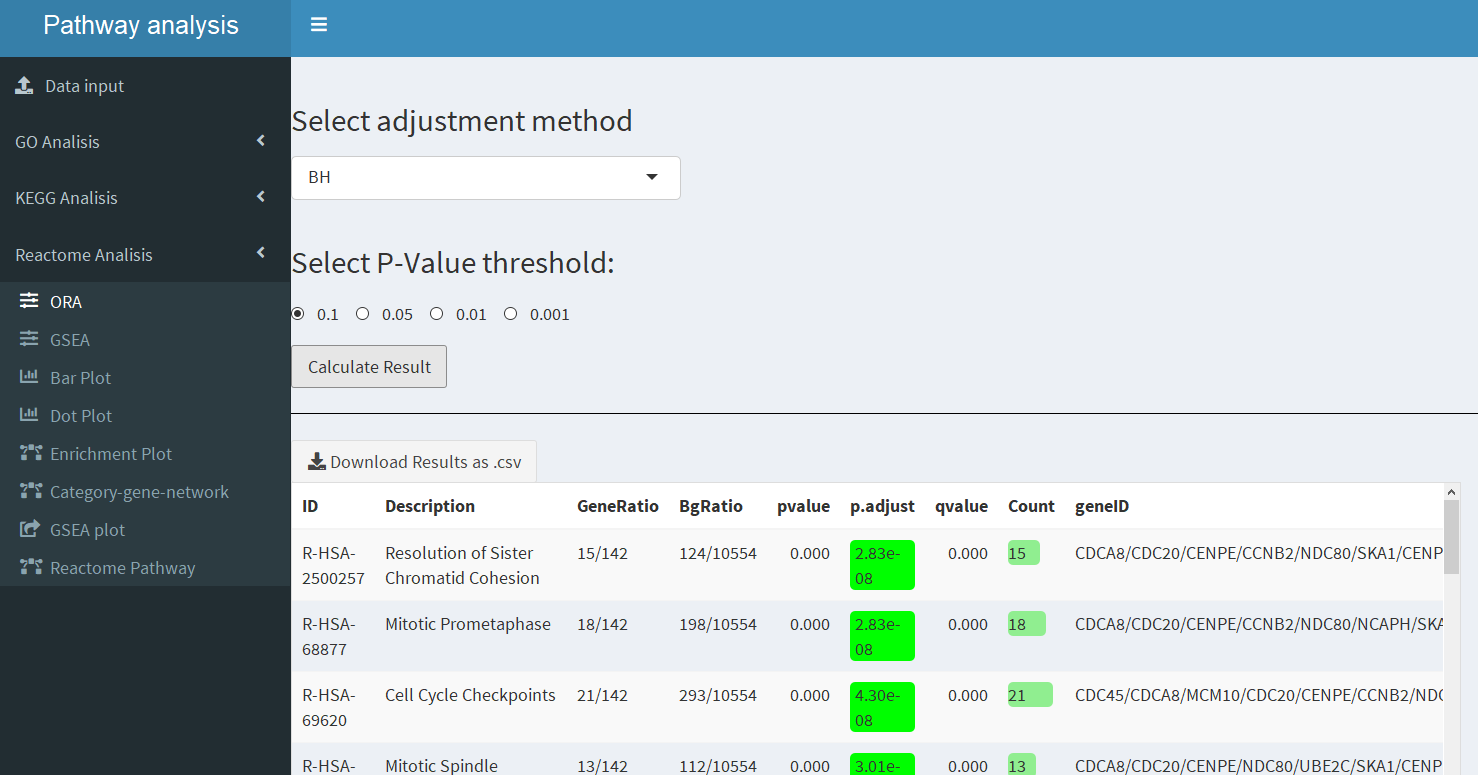
\includegraphics[width=0.9\textwidth]{App_F10_Items_Reactome_ORA.png} 
\caption{El resultat d'anàlisi ORA. Reactome.}
\end{figure}

\subsection{GSEA}
\subsubsection{GO}
El mètode GSEA per a termes GO es calcula amb la funció \helvetica{gseGO()} del paquet \helvetica{clusterProfiler}. 

\begin{lstlisting}[language=R]
gseGO(geneList, ont = "BP", OrgDb, keyType = "ENTREZID",
exponent = 1, nPerm = 1000, minGSSize = 10, maxGSSize = 500,
pvalueCutoff = 0.05, pAdjustMethod = "BH", verbose = TRUE,
seed = FALSE, by = "fgsea")
\end{lstlisting}

L'usuari pot elegir l'ontologia GO, el \textit{cut-off} del valor P i el mètode d'ajustament.
\begin{figure}[H]
\centering
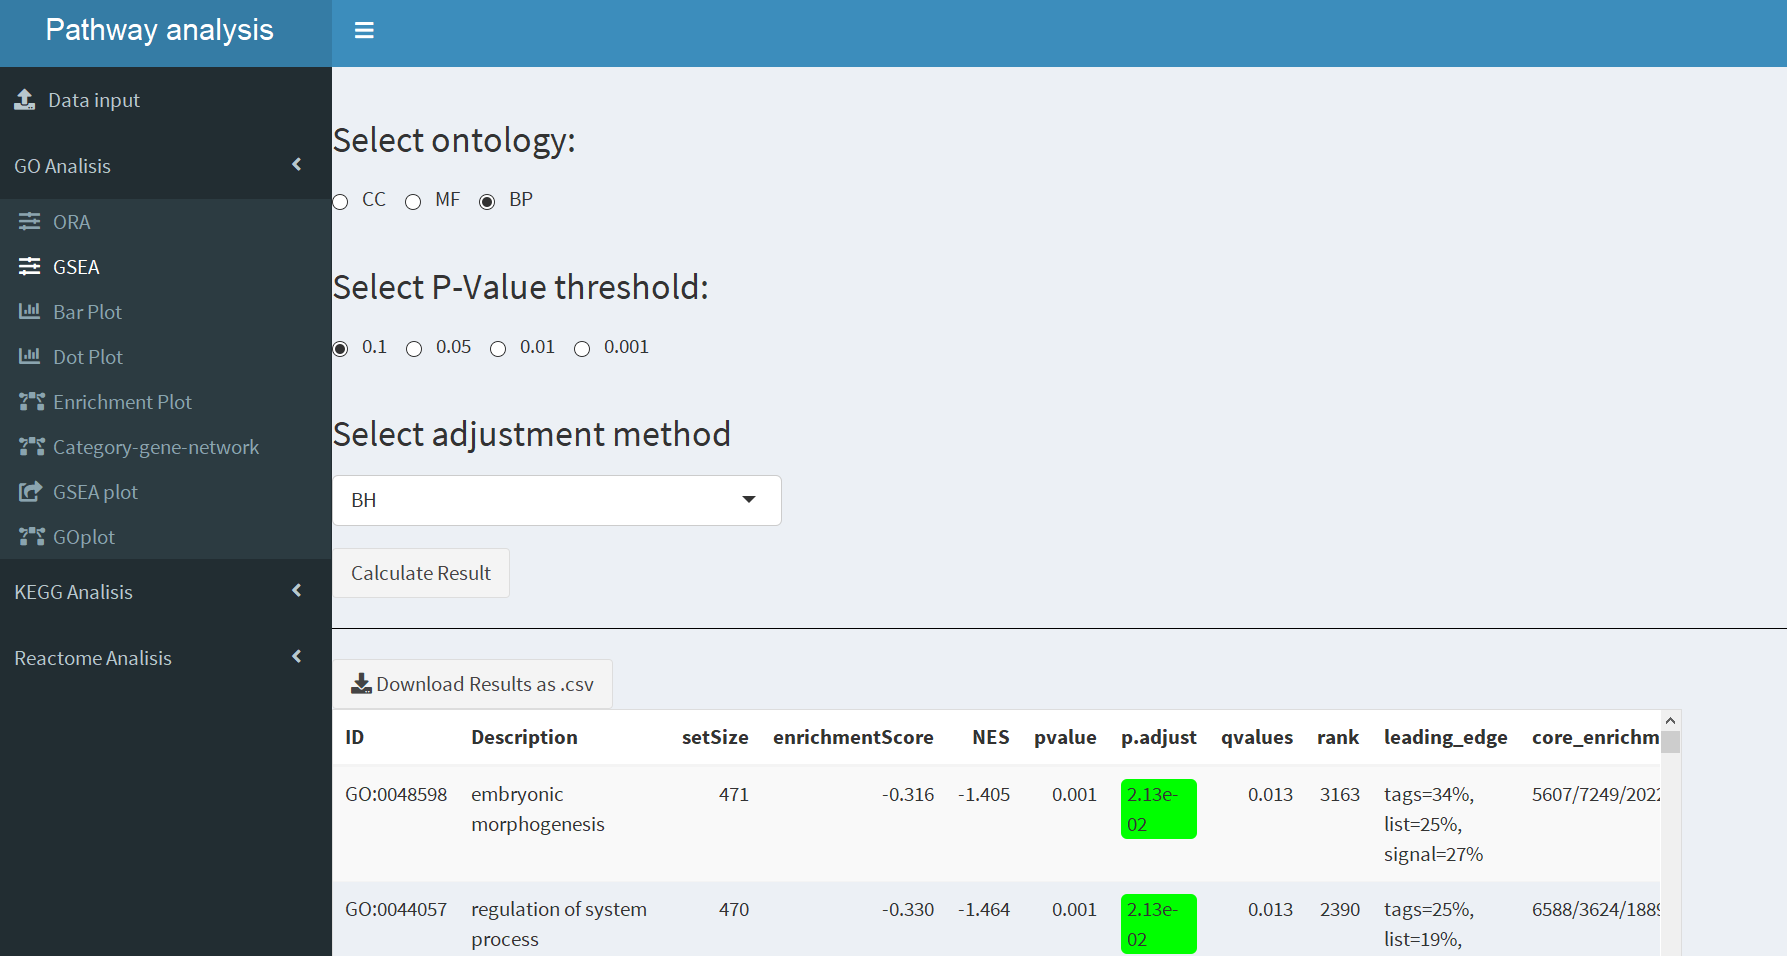
\includegraphics[width=0.9\textwidth]{App_F11_Items_GO_GSEA.png} 
\caption{El resultat de l'anàlisi GSEA. GO.}
\end{figure}


\subsubsection{KEGG}
De la mateixa manera es calcula GSEA amb la funció \helvetica{gseKEGG()} del paquet \helvetica{clusterProfiler}:

\begin{figure}[H]
\centering
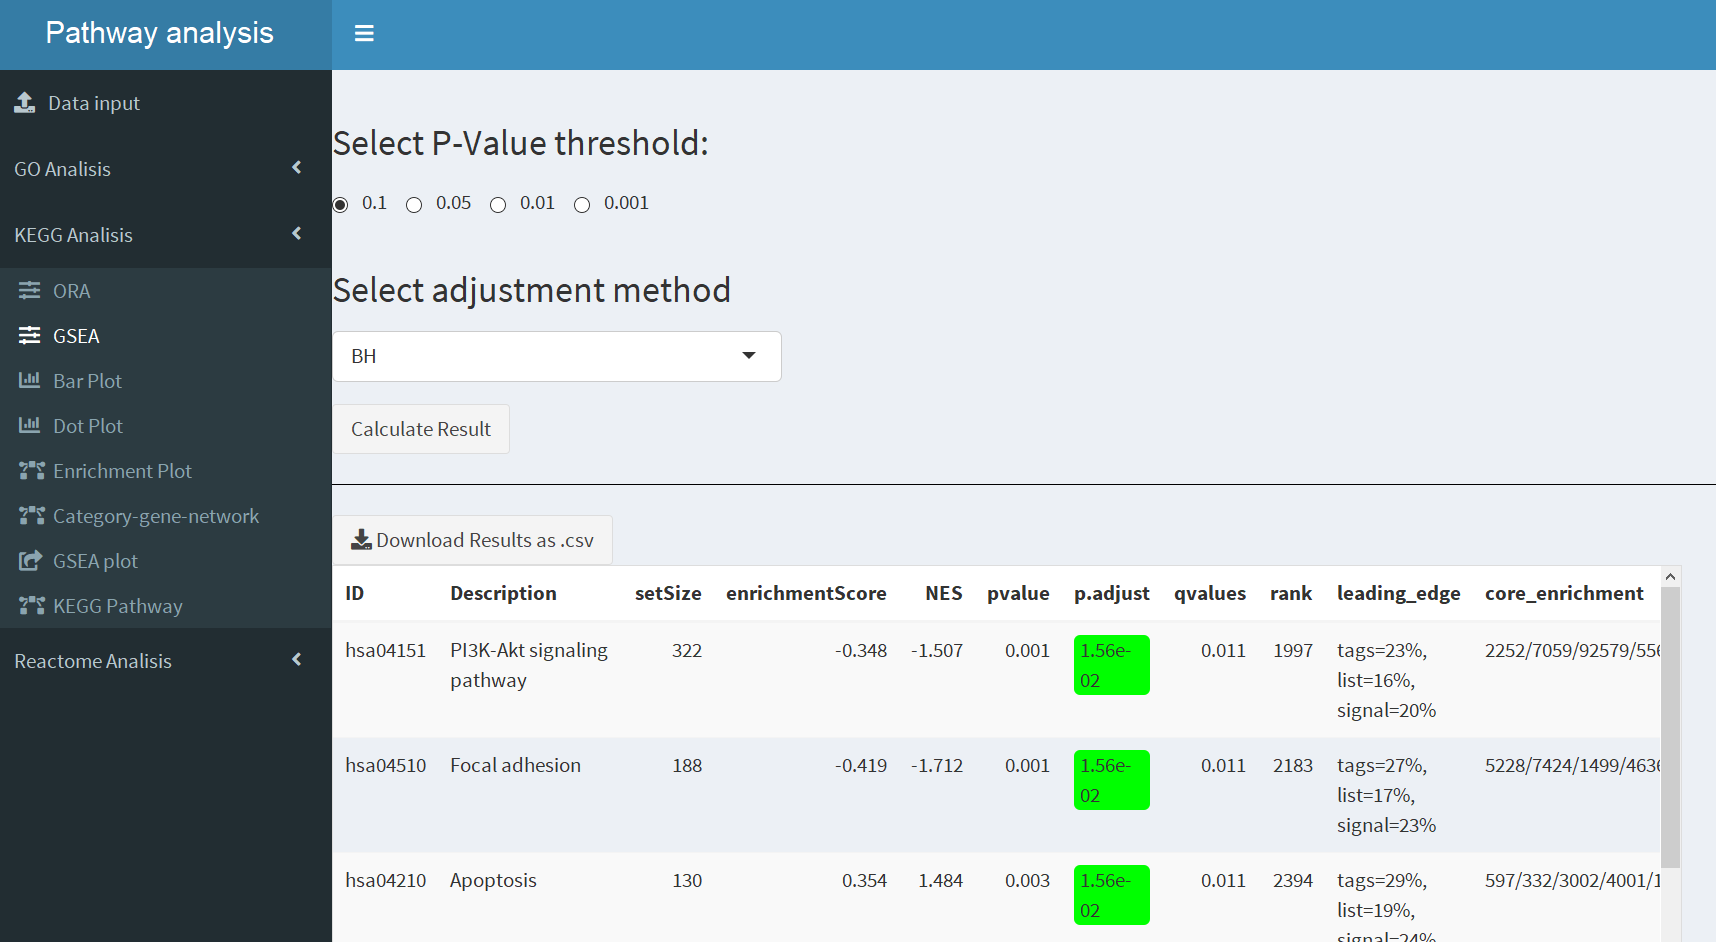
\includegraphics[width=0.9\textwidth]{App_F12_Items_KEGG_GSEA.png} 
\caption{El resultat de l'anàlisi GSEA. KEGG.}
\end{figure}

\subsubsection{Reactome}
Per completar l'anàlisi l'usuari pot calcular GSEA per a base de dades Reactome. Com als altres casos utilitzo el paquet \helvetica{clusterProfiler} i específicament la funció \helvetica{gsePathway()}

\begin{figure}[H]
\centering
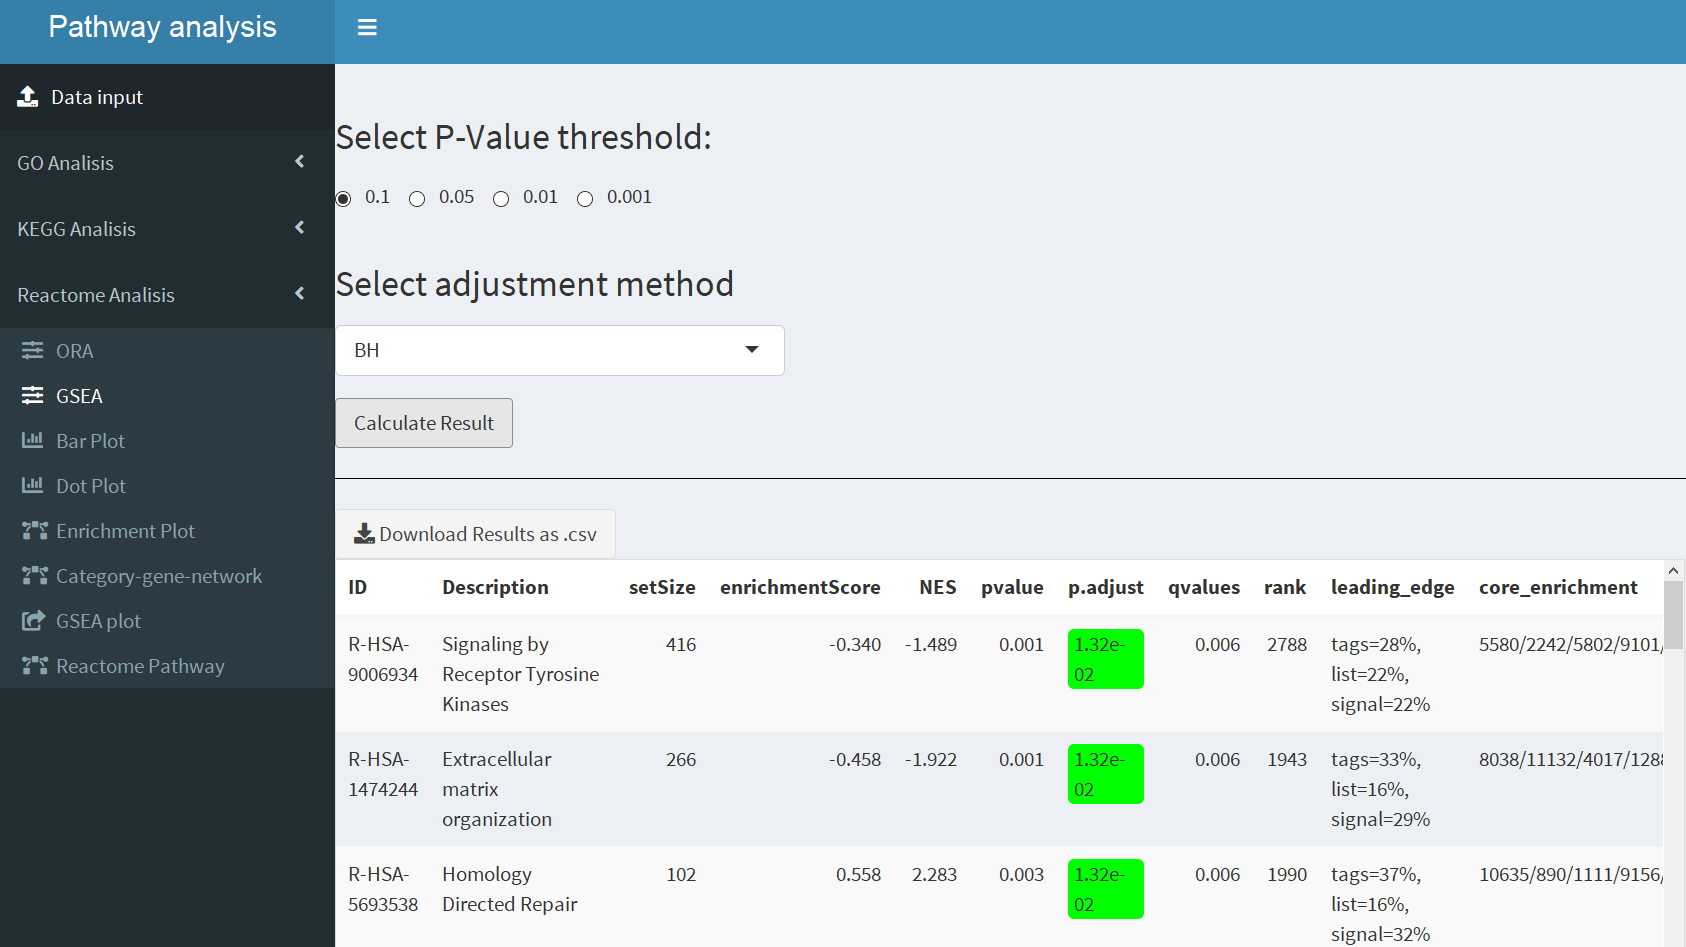
\includegraphics[width=0.9\textwidth]{App_F13_Items_RA_GSEA.png} 
\caption{El resultat d'anàlisi GSEA. Reactome.}
\end{figure}

\subsection{Bar-Plots}
Els resultats de \helvetica{enrichGO}, \helvetica{enrichKEGG} i \helvetica{enrichPathway} es poden visualitzar amb el gràfic de barres. L'usuari pot elegir el nombre de les categories visualitzades entre 2 i 30. Es dona l'opció per descarregar el gràfic en format .png.

\begin{figure}[H]
\centering
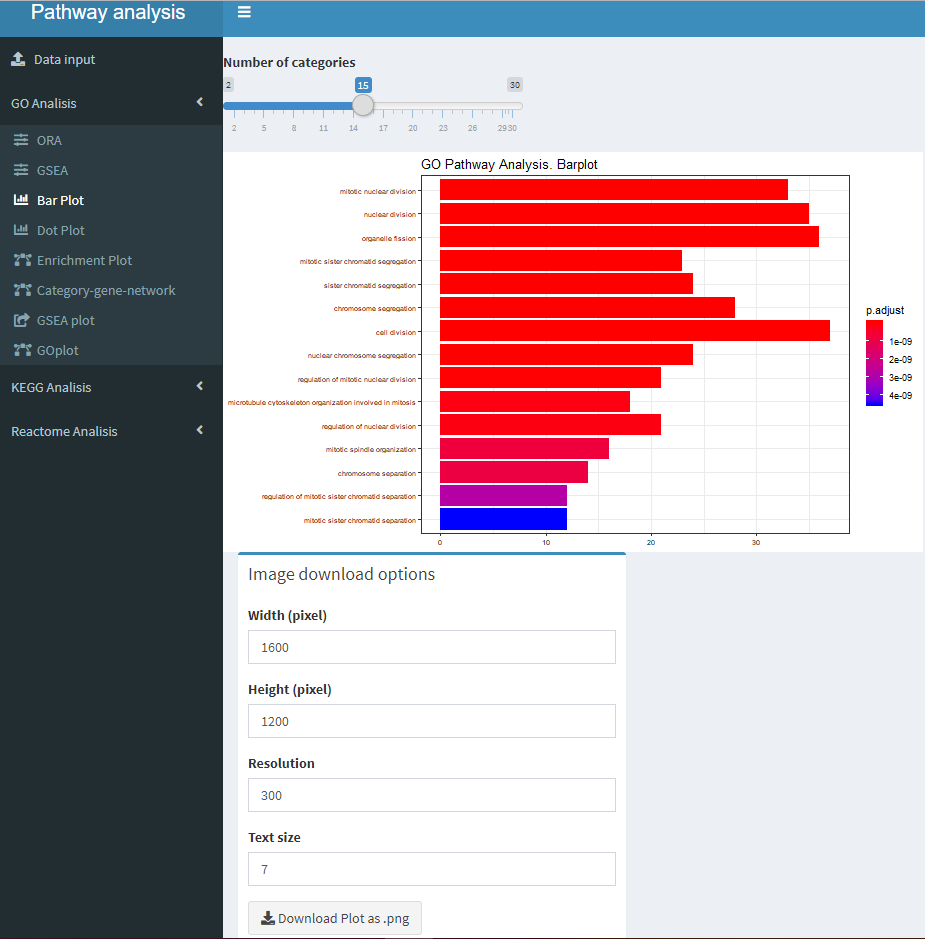
\includegraphics[width=0.9\textwidth]{App_F14_Items_GO_BarPlot.png} 
\caption{Bar-Plot. GO.}
\end{figure}

\subsection{Dot-Plots}

El \textit{dot plot} visualitza addicionalment el \textit{gen ratio}. També aquí l'usuari pot seleccionar el nombre de categories.


\begin{figure}[H]
\centering
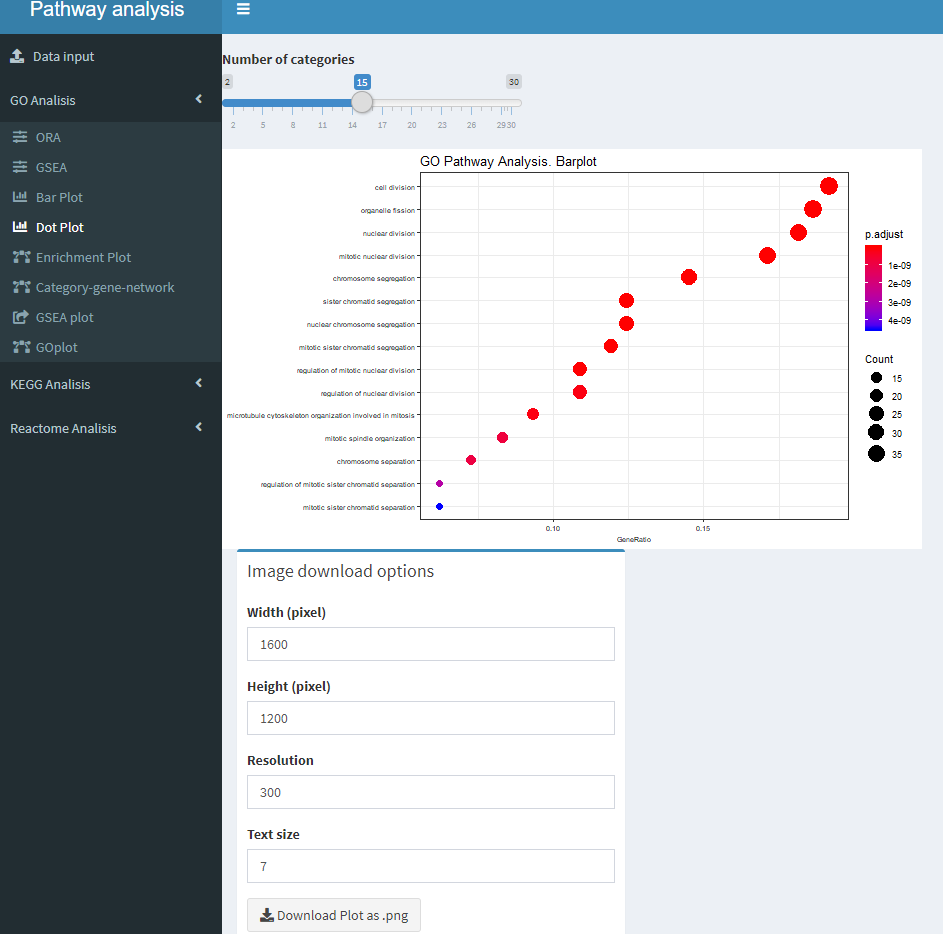
\includegraphics[width=0.9\textwidth]{App_F15_Items_GO_DotPlot.png} 
\caption{Bar-Plot. GO.}
\end{figure}

\subsection{Enrichment Plots}

\begin{figure}[H]
\centering
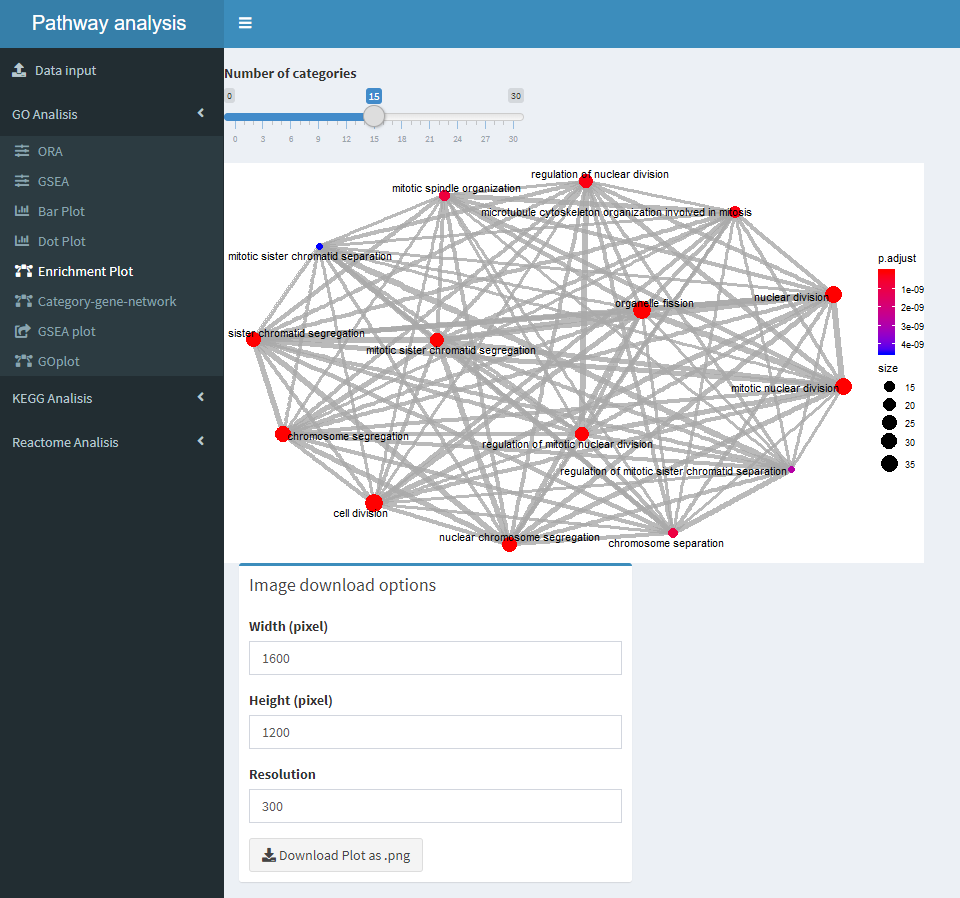
\includegraphics[width=0.9\textwidth]{App_F16_Items_GO_Emap.png} 
\caption{Bar-Plot. GO.}
\end{figure}

\subsection{Category-Gene-Network Plot}

\begin{figure}[H]
\centering
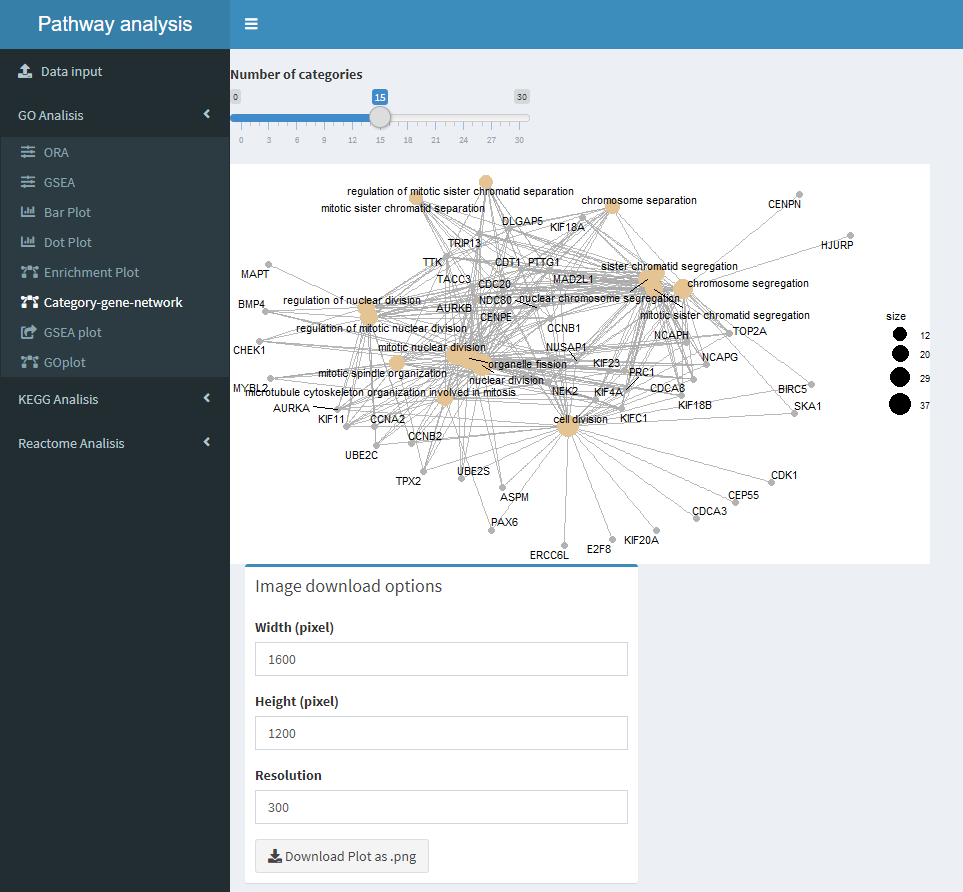
\includegraphics[width=0.9\textwidth]{App_F17_Items_GO_CnetPlot.png} 
\caption{Category-Gene-Network Plot. GO.}
\end{figure}

\subsection{GSEA Plot}
L'usuari pot visualitzar una de les categories disponibles via \textit{dropdown list}. El llistat inclou totes les rutes generades durant l'anàlisi GSEA en els apartats \textit{Go Analysis}$\rightarrow$\textit{GSEA}; \textit{KEGG}$\rightarrow$\textit{GSEA}
\begin{figure}[H]
\centering
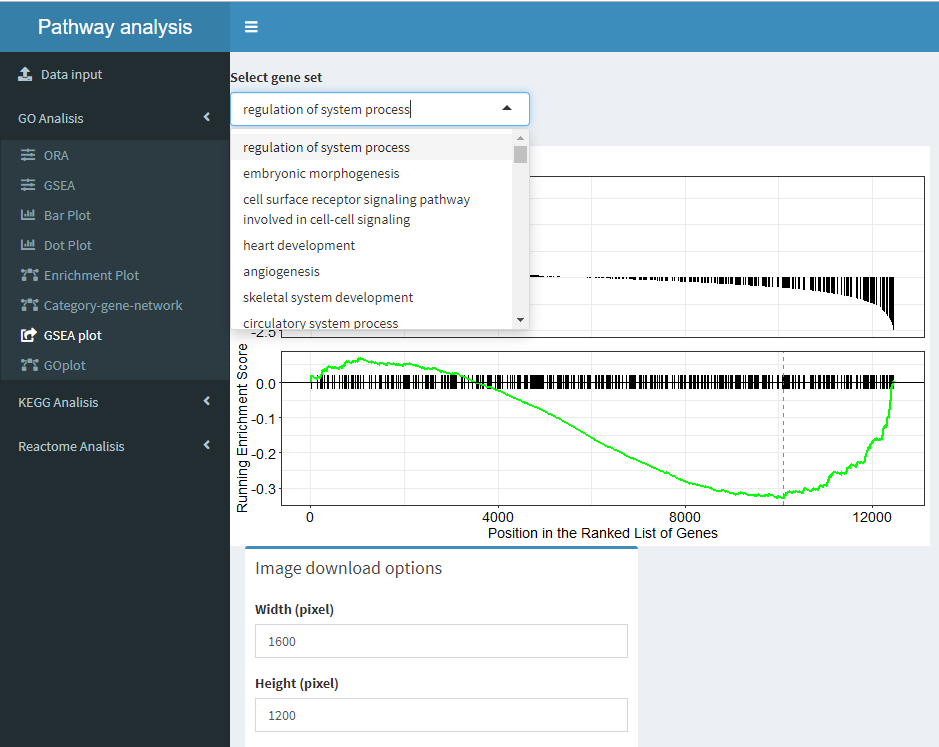
\includegraphics[width=0.9\textwidth]{App_F18_Items_GO_GSEA_Plot.png} 
\caption{GSEA Plot. GO.}
\end{figure}


\section{L'anàlisi específic de GO, KEGG i Reactome}

\label{sec:ASpec}


\subsection{GO Plot}

\begin{figure}[H]
\centering
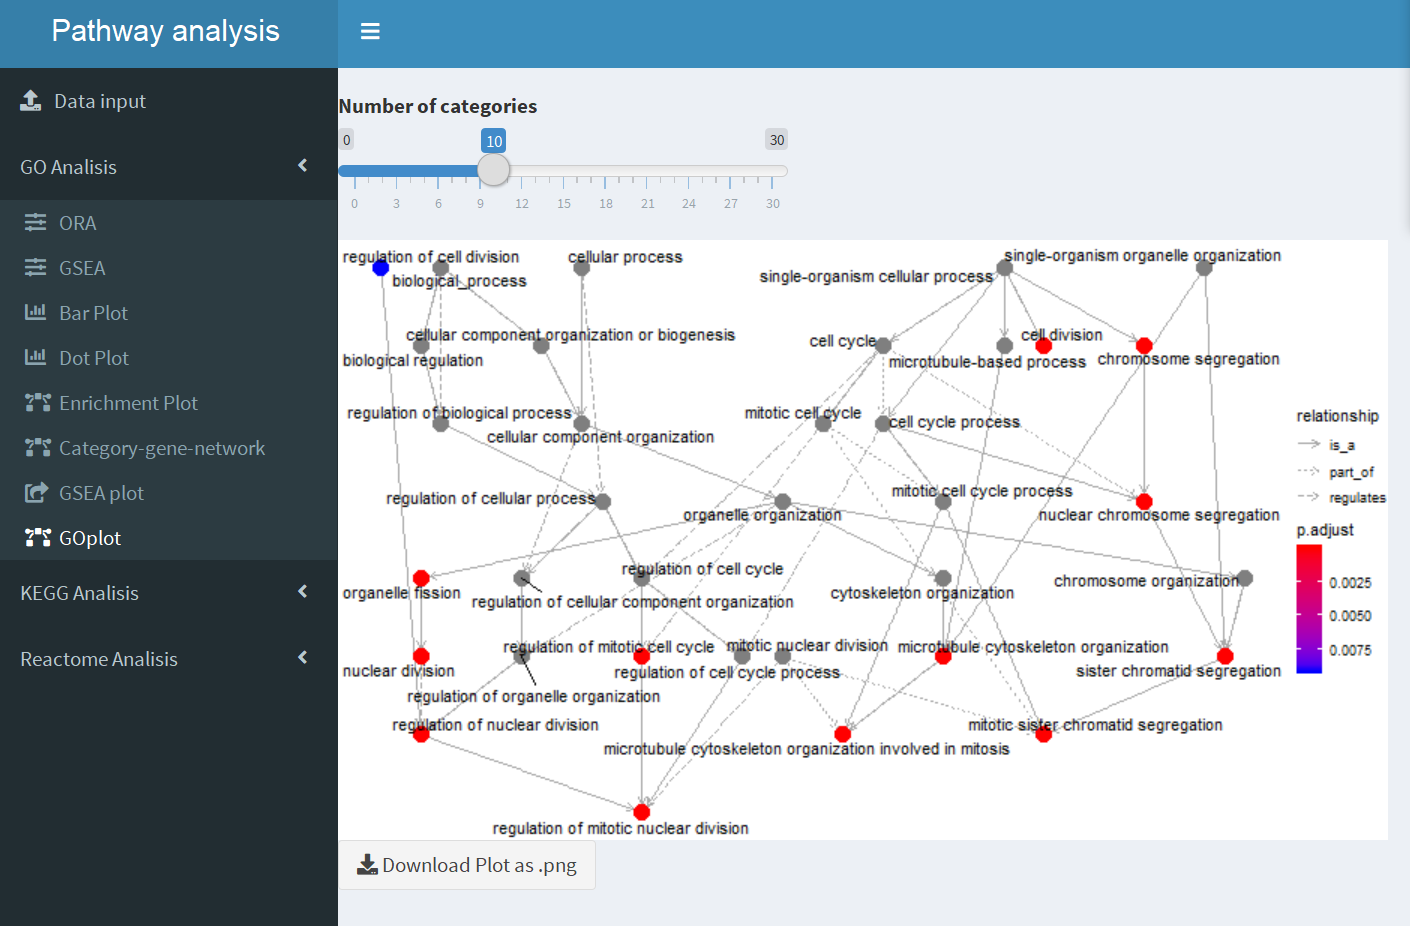
\includegraphics[width=0.9\textwidth]{App_F19_Items_GO_GOPlot.png} 
\caption{GO Plot}
\end{figure}

\subsection{KEGG Pathway}


\begin{figure}[H]
\centering
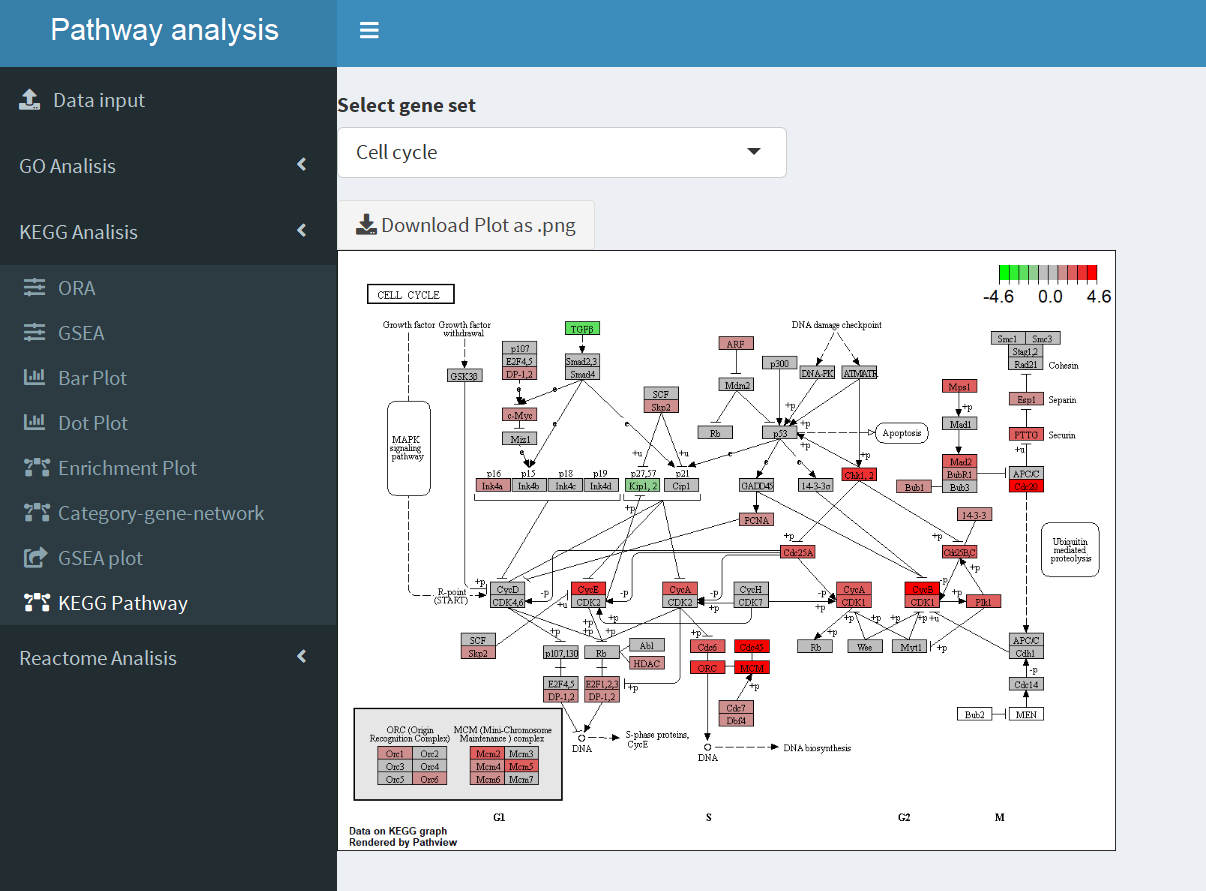
\includegraphics[width=0.9\textwidth]{App_F20_Items_KEGG_KEGGPathway.png} 
\caption{KEGG pathway}
\end{figure}

\subsection{Reactome Pathway}

\begin{figure}[H]
\centering
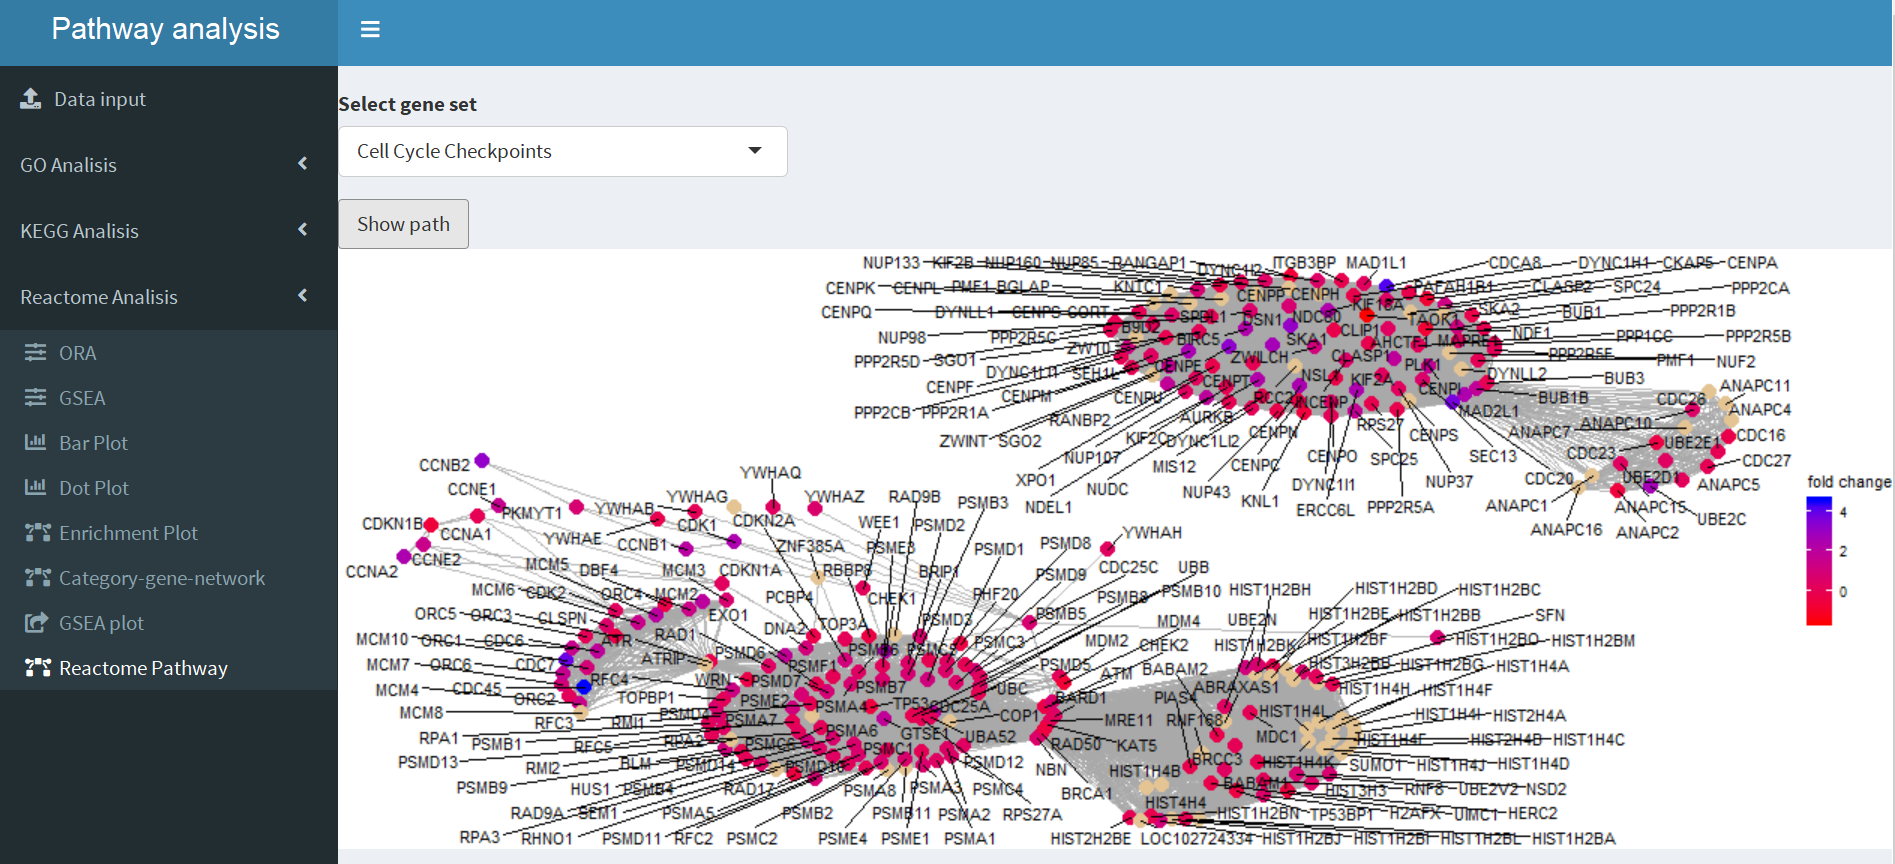
\includegraphics[width=0.9\textwidth]{App_F21_Items_RA_RAPathway.png} 
\caption{Reactome pathway}
\end{figure}


\section{Manual i les ajudes del programa}

Per facilitar l'ús de l’aplicació he pensat com es podria fer de manera més intuïtiva possible. Primer cal destacar que com a llengua de manual he elegit l’anglès per poder fer l'ús de l'aplicació el més inclusiu possible. Segon, l'usuari pot accedir tant al manual com a l'ajuda, que es guarden en arxius .Md separats. Per accedir al manual l'usuari ha de clicar al símbol d’interrogació a prop del títol \textbf{Pathway analysis}:
\begin{figure}[H]
\centering
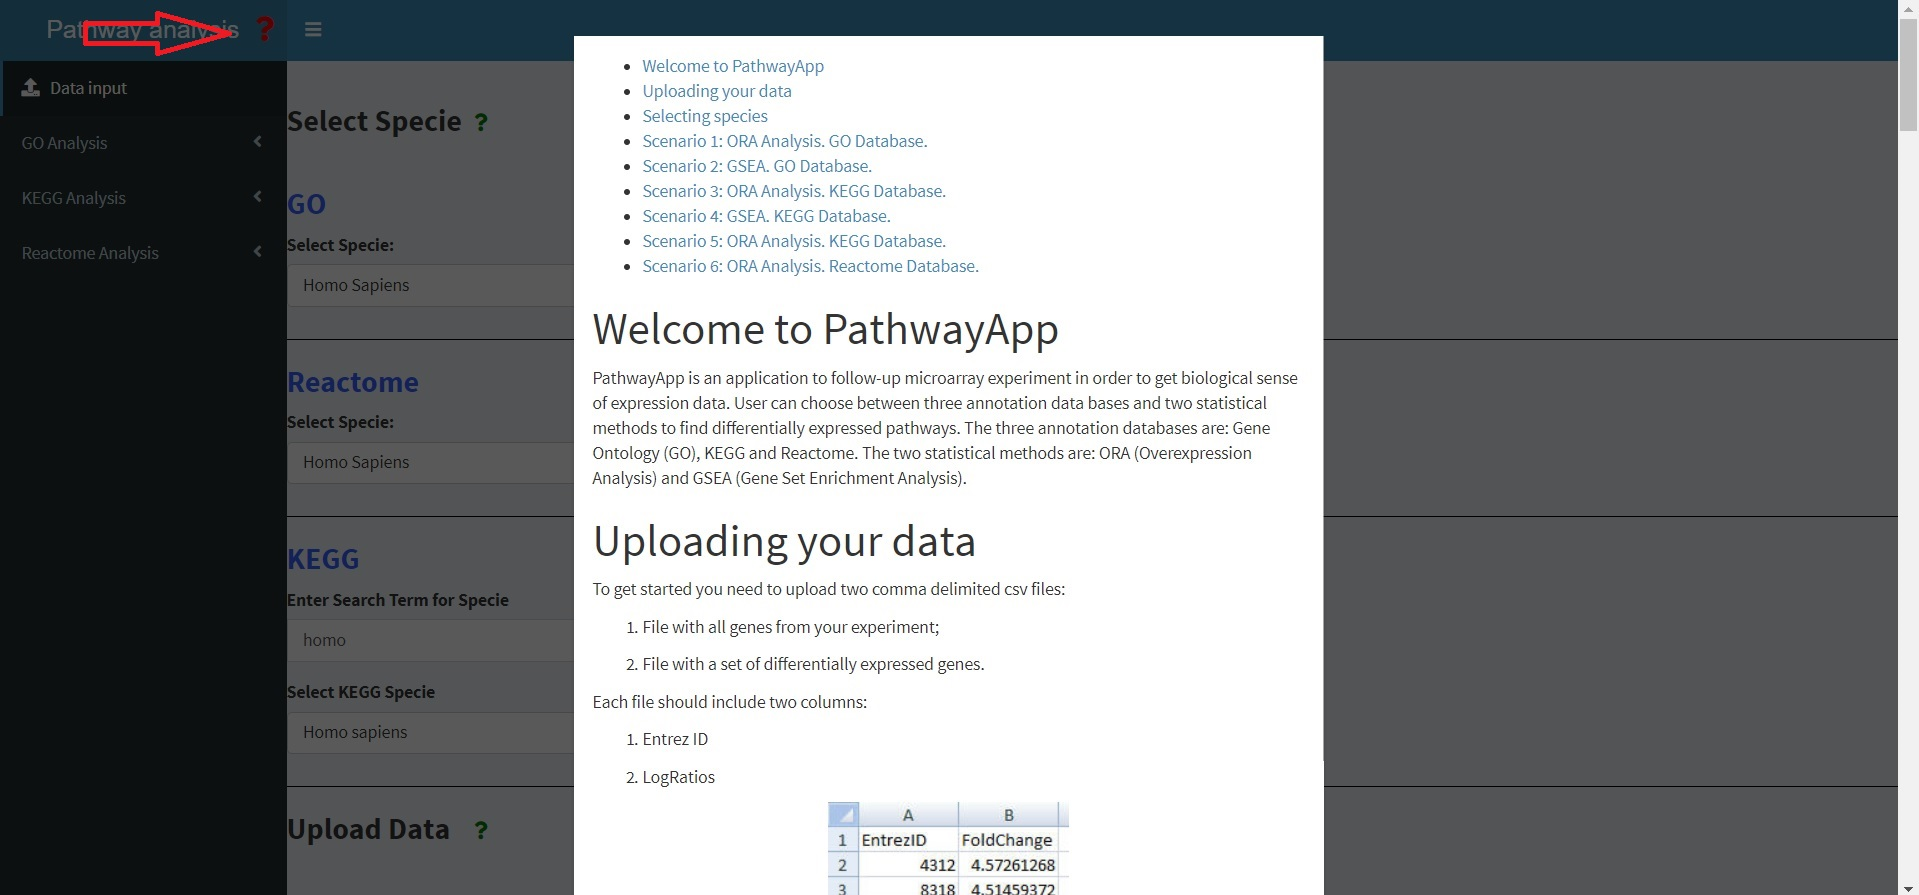
\includegraphics[width=1\textwidth]{Manual.jpg} 
\caption{Manual per a aplicació}
\end{figure}

Com es veu hi ha apartats diferents. Depenent dels objectius de l'usuari, aquest pot seleccionar l'apartat que més l'interessi. Així, si l'usuari vol fer l'anàlisi ORA amb l'anotació KEGG pot navegar en la secció |textbf{Scenario 3: ORA Analysis. KEGG Database}. 

\begin{figure}[H]
\centering
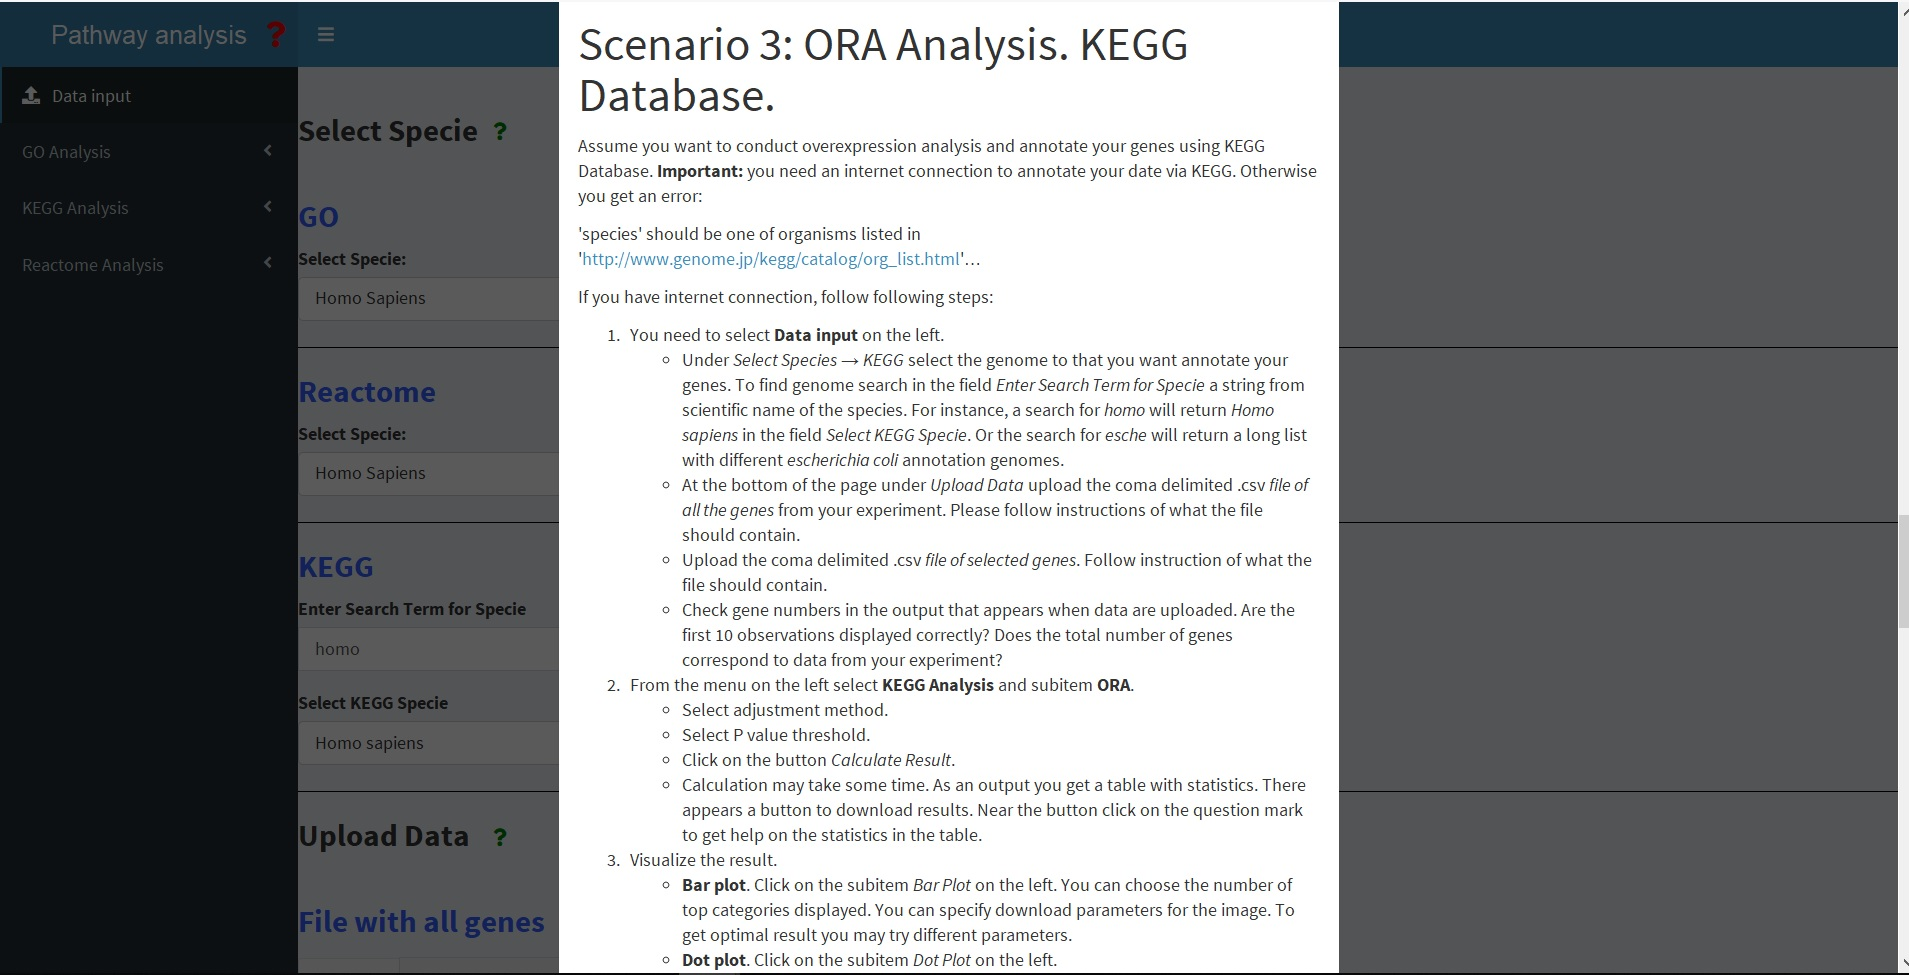
\includegraphics[width=1\textwidth]{Manual2.jpg} 
\caption{Manual per a l'anàlisi ORA amb l'anotació KEGG}
\end{figure}


També, l'usuari pot accedir a l'ajuda clicant als símbols d'interrogació distribuïts per l’aplicació en els llocs que penso que poden generar dubtes. 

Per fer-ho possible s'utilitza el paquet \helvetica{shinyhelper} que s'instal·la en executar la funció \helvetica{runPathwayApp()}.

\begin{figure}[H]
\centering
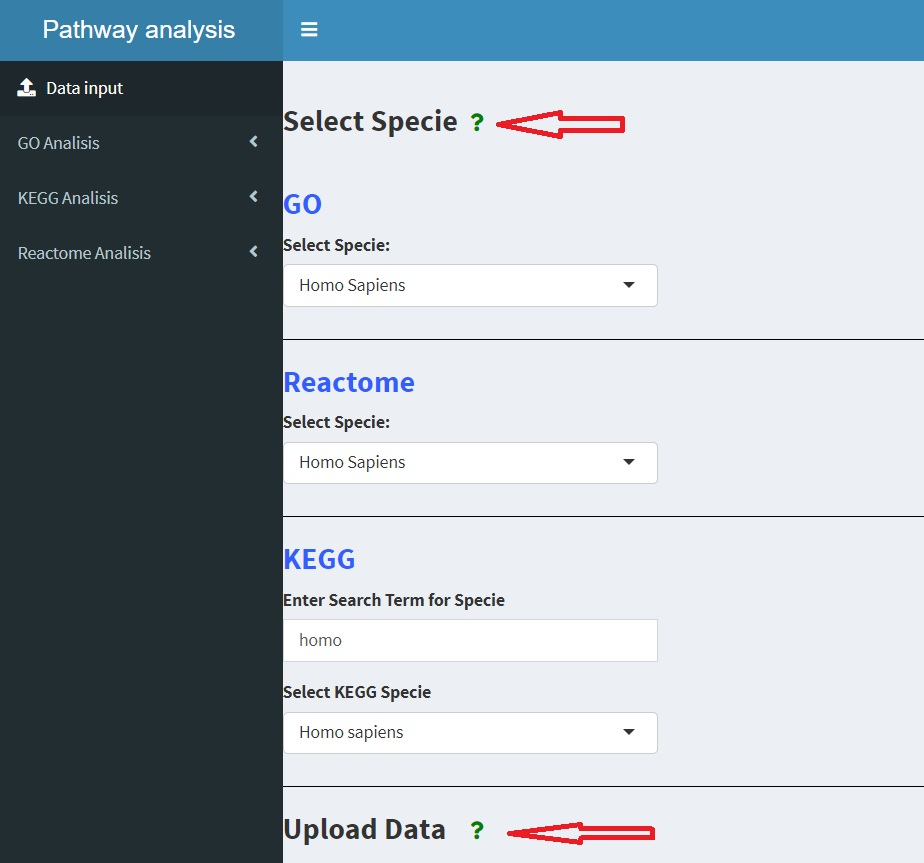
\includegraphics[width=0.7\textwidth]{Help_Data_Input.jpg} 
\caption{Senyals d'ajuda}
\end{figure}

El clic en aquests senyals fa que aparegui una finestreta amb la informació d'ajuda.

Aquí hi ha informació de l'apartat \textbf{Data Input}:

\begin{figure}[H]
\centering
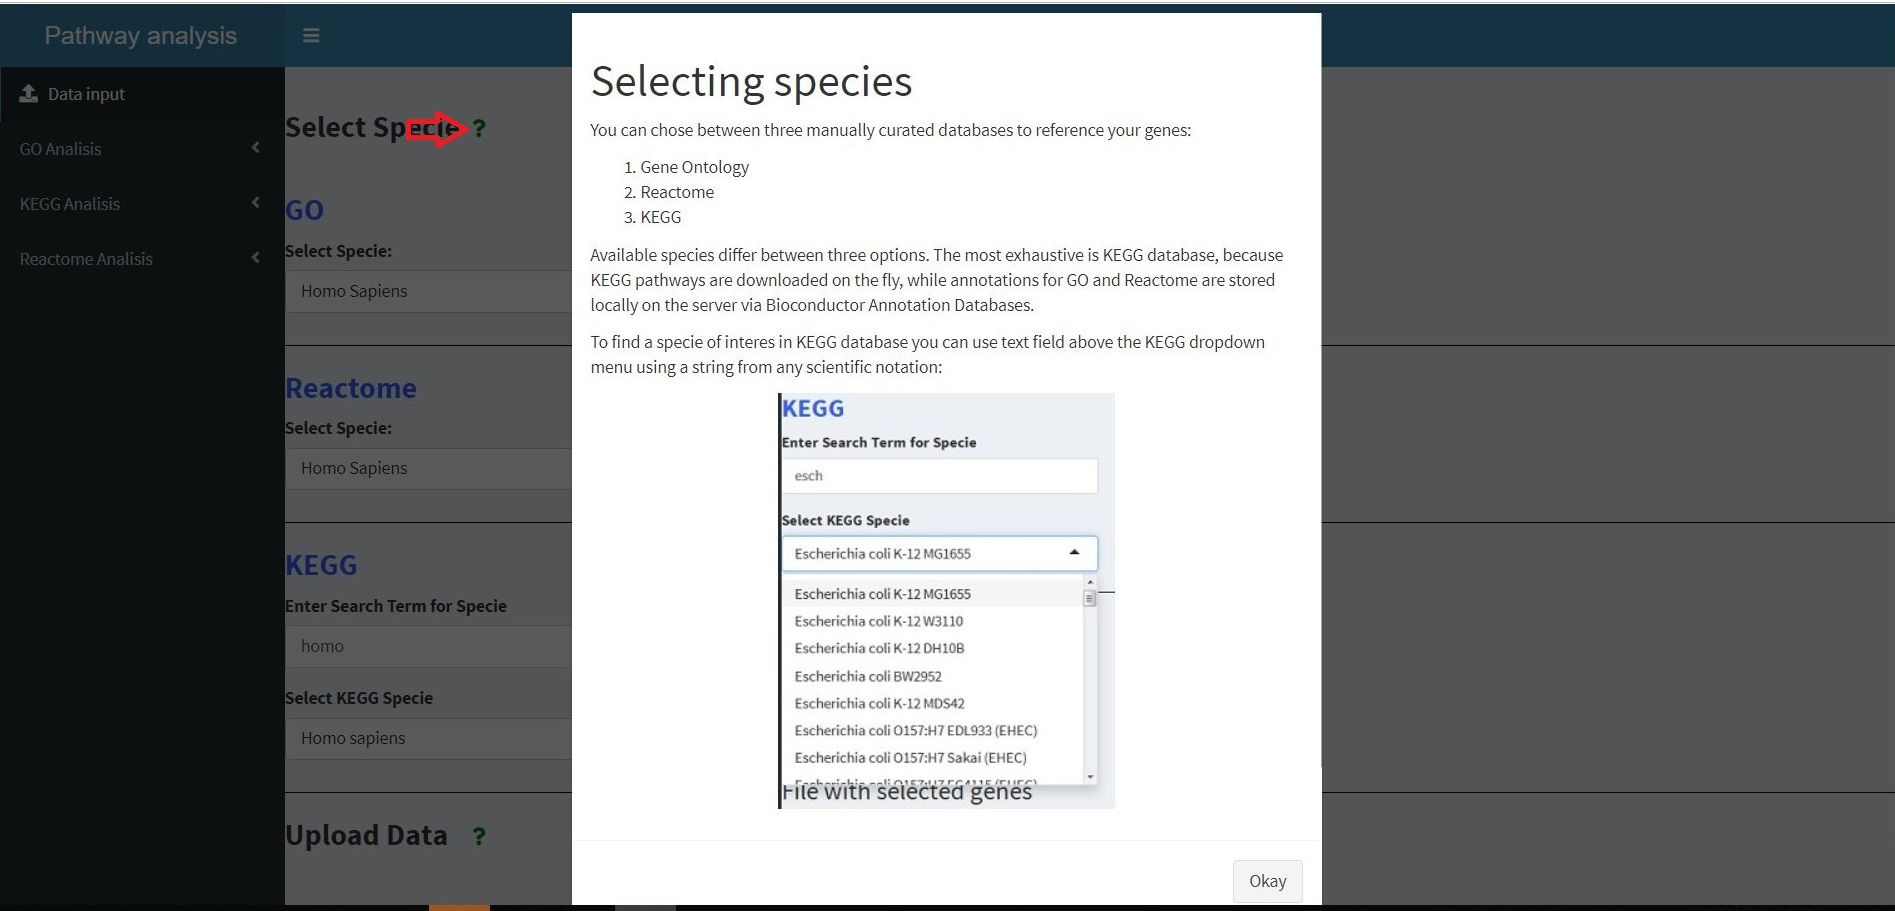
\includegraphics[width=0.9\textwidth]{Help_Specie.jpg} 
\caption{Ajuda per a l'elecció de l'espècie}
\end{figure}

\begin{figure}[H]
\centering
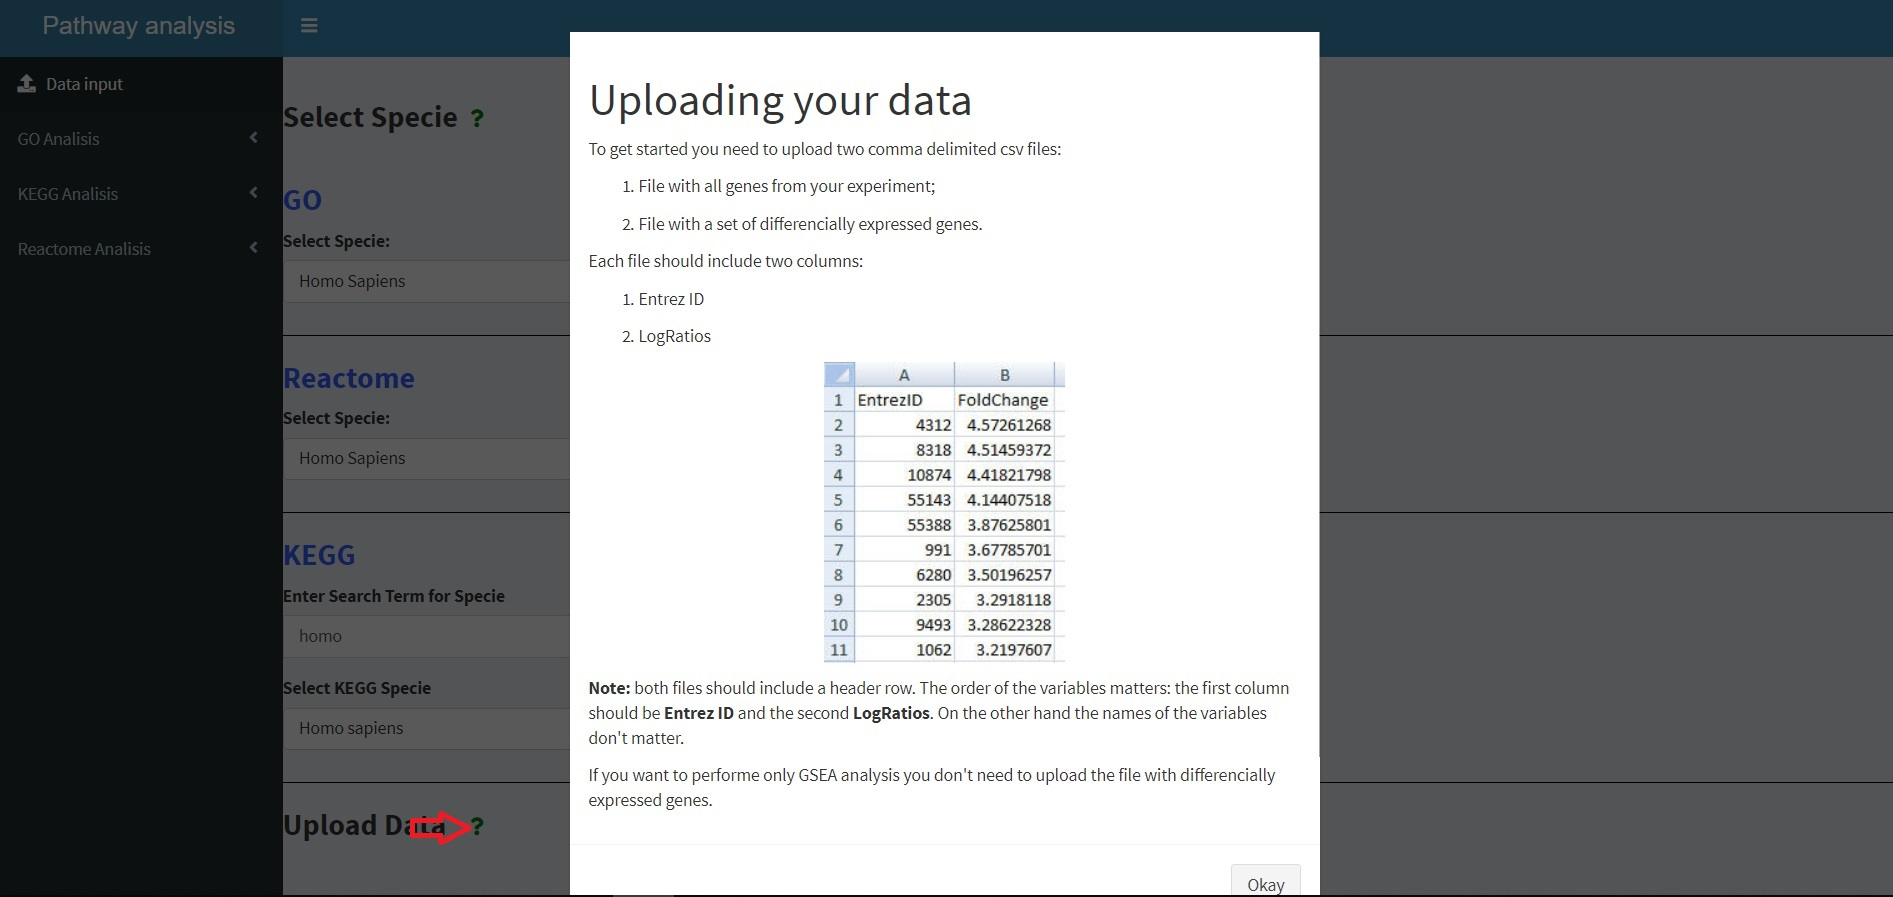
\includegraphics[width=0.9\textwidth]{Help_Upload_Data.jpg} 
\caption{Ajuda per pujar les dades}
\end{figure}

Les informacions per a l'apartat ORA són les següents:

\begin{figure}[H]
\centering
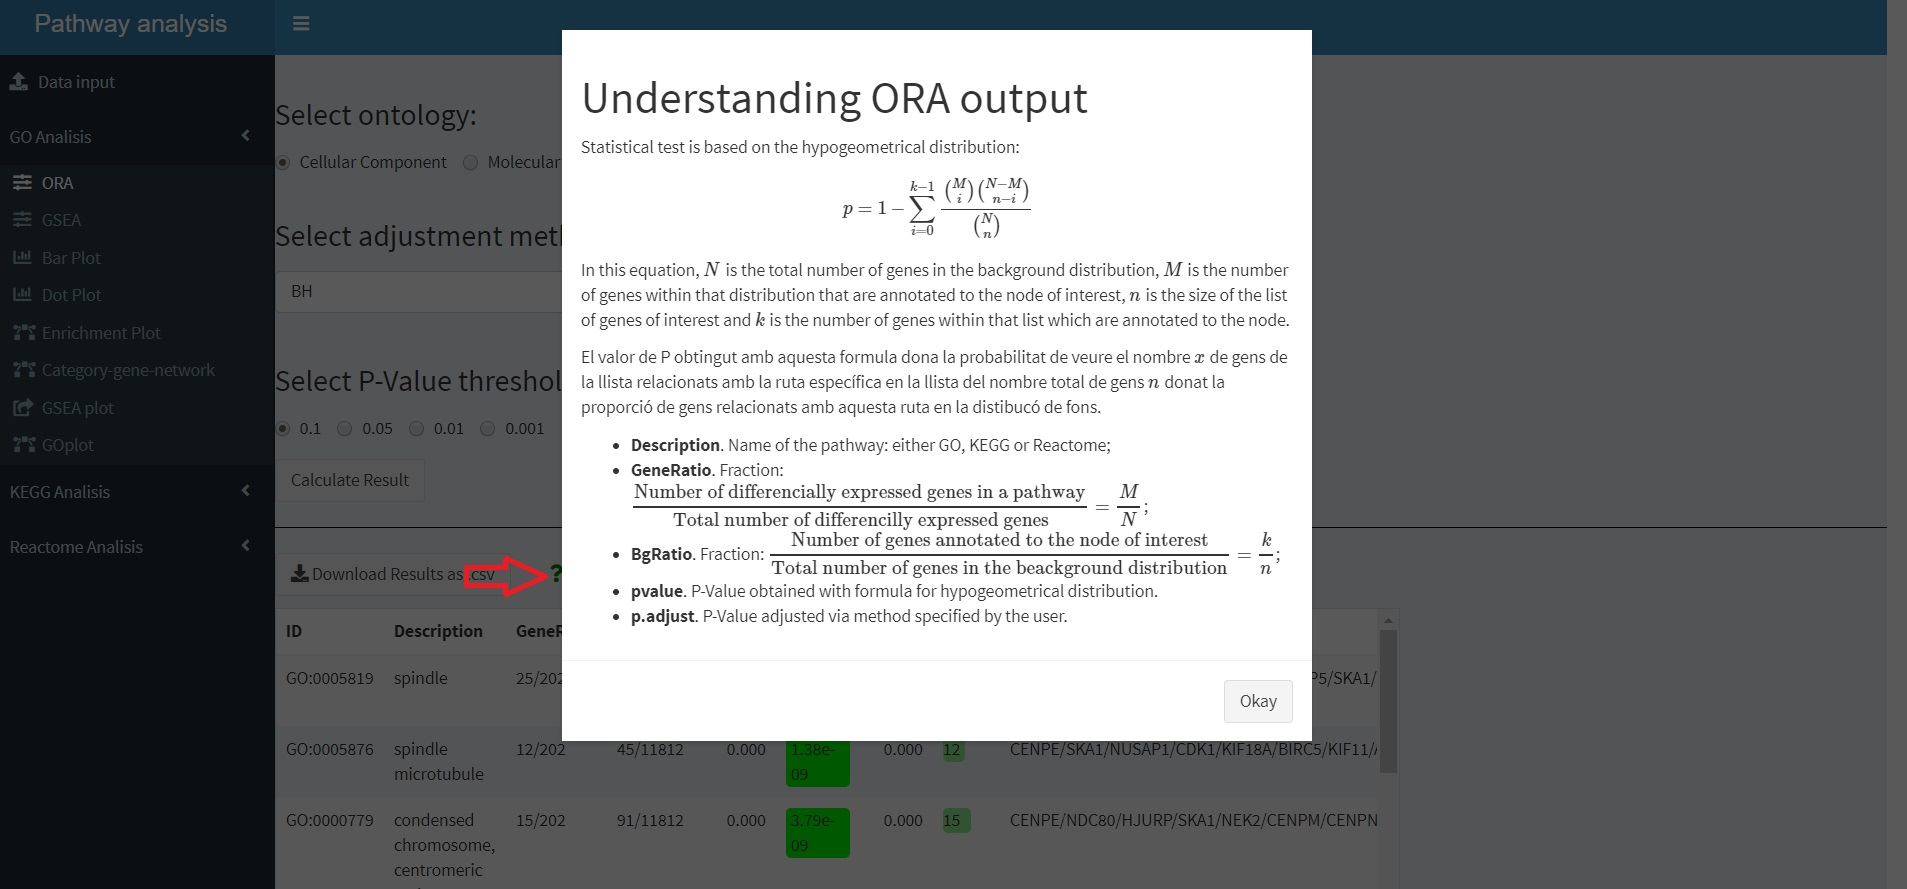
\includegraphics[width=0.9\textwidth]{Help_ORA_output.jpg} 
\caption{Infromació per la interpretació d'anàlisi ORA}
\end{figure}
Aquí cal destacar que les fòrmules, depenent de l'ordinador, no apareixen degudament en el RStudio Browser. Sí que apareixen bé quan l'aplicació s'obre via l’internet browser. L'usuari ha de tenir connexió amb internet perquè l'aplicació pugui descodificar la fòrmula via MathJax. Encara no he trobat la causa per la qual el Rstudio Browser en alguns ordinadors no visualitza bé les fòrmules. Pot ser un problema amb Java, que s'ha d'actualitzar? Ho estic investigant.

\begin{figure}[H]
\centering
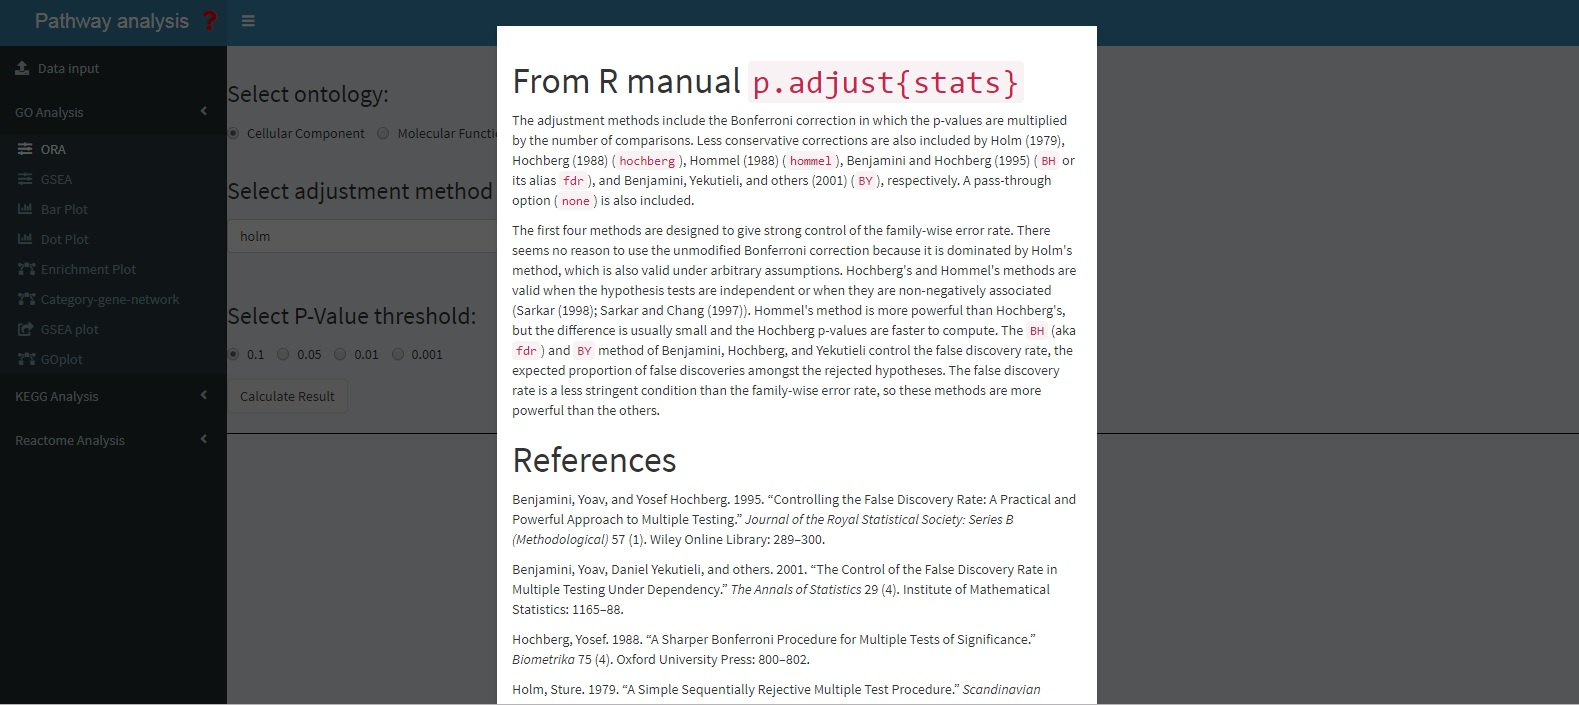
\includegraphics[width=0.9\textwidth]{Help_pAdjustMethod.jpg} 
\caption{L'ajuda per a la selecció del mètode d'ajustament}
\end{figure}


\begin{figure}[H]
\centering
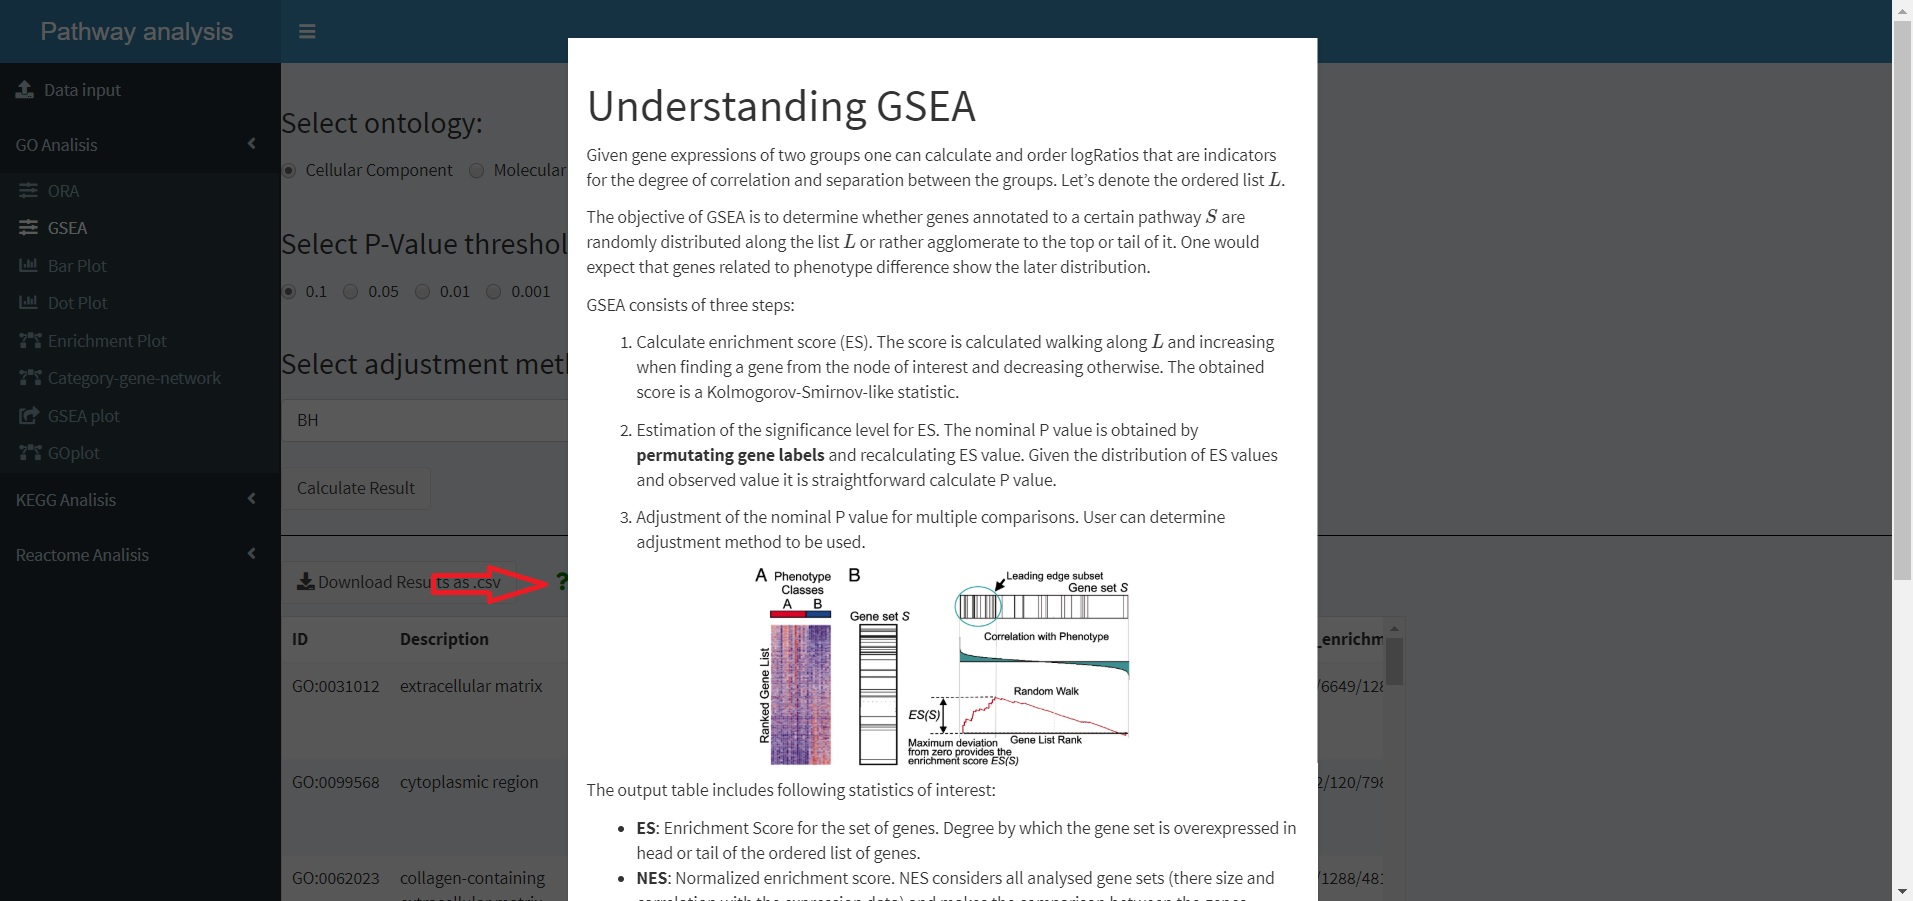
\includegraphics[width=0.9\textwidth]{Help_GSEA_output.jpg} 
\caption{Ajuda per la interpretació de GSEA}
\end{figure}


\section{Validació dels resultats}
\label{sec:ValRes}

L’anàlisi de les rutes representa l’últim pas de l’anàlisi d’expressions. Per dur a terme l’anàlisi de rutes és necessari tenir unes dades que ja estiguin processades prèviament (normalització, càlcul de les LogRatios, ajustament dels gens repetits a l’array, selecció dels gens diferencialment expressats, etc.). Les dades de \href{https://www.ncbi.nlm.nih.gov/geo/}{GEO (Gene Expression Omnibus)} estan però disponibles com a màxim en format normalitzat. Caldria doncs fer una anàlisi per arribar a un llistat de gens diferencialment expressats amb les logRatios per tots els gens de la mostra. Fer això no seria cap problema i de fet ho he fet per altres estudis. El problema és que arribo a resultats diferents dels resultats dels estudis d’on provenen les dades (i no parlo de l’anàlisi de les rutes sinó ja del càlcul de les logRatios). Per tant les dades que entraria a l’aplicació serien diferents de les dades de l’estudi i lògicament amb aquesta comprovació no comprovo el que realment m’interessa. Podria, doncs, dedicar-me a trobar el motiu pel qual els resultats són diferents, però fer totes aquestes comprovacions prèvies no té a veure amb l’objecte del meu treball de màster, l’anàlisi de les rutes. Per tant he procedit a contactar el meu profesor per si tindria (o coneixeria) dades preprocessades fins a un llistat de gens amb logRatios i amb el set de gens diferencialment expressats, per tal que les pugui utilitzar en la meva aplicació. El meu professor m'ha redirigit, entre altres enllaços molt útils, al seu repositori en \href{https://github.com/alexsanchezpla?tab=repositories}{github.com}. 


\begin{center}
\begin{tabular}{||c | c | c | c | c ||} 
\hline 
Estudi & GEO ID & Espècie & Tipo d'experiment & Font \\ [0.5ex] 
\hline\hline
\cite{schmidt2008humoral} & \href{https://www.ncbi.nlm.nih.gov/geo/query/acc.cgi?acc=GSE11121}{GSE11121}& Homo sapiens & Microarrays & \href{https://bioconductor.org/packages/release/bioc/html/DOSE.html}{Paquet \helvetica{DOSE} de Bioconductor}\\
\hline
\cite{li2017zbtb7b} & \href{https://www.ncbi.nlm.nih.gov/geo/query/acc.cgi?acc=GSE100924}{GSE100924}& Mus musculus & Microarrays & \href{https://github.com/alexsanchezpla/StatisticalAnalysisOfMicroarrayData}{Github Sanchez Pla} \\ 
\hline
\cite{farmer2005identification} & \href{https://www.ncbi.nlm.nih.gov/geo/query/acc.cgi?acc=GSE1561}{GSE1561}&Homo sapiens& Microarrays & \href{https://github.com/alexsanchezpla/Ejemplo_de_MDA_con_Bioconductor}{Github Sanchez Pla} \\ 
\hline
\cite{hengel2003cutting} & \href{https://david.ncifcrf.gov/helps/demo1.txt}{DAVID Demo List 1}&Homo sapiens& Microarrays & \href{https://david.ncifcrf.gov/content.jsp?file=FAQs.html}{DAVID} \\ 
\hline
\end{tabular}
\end{center}

Les dades de \cite{schmidt2008humoral}, que s'utilitzen en els vignettes de \helvetica{clusterProfiler} i \helvetica{ReactomePA}, ja les he mostrat en gran part a dalt quan explicava el contingut de l'aplicació. Els resultats obtinguts amb l'aplicació són iguals als resultats en els vignettes mencionats. Procediré doncs amb l'exemple basat en les dades de \cite{li2017zbtb7b} .

\subsection{Exemple d'anàlisi 1. GEO: GSE100924}

Les dades d'estudi \cite{li2017zbtb7b} són ja preprocessades per Ricardo Gonzalo Sanz i Sanchez Pla i estan disponibles a \href{https://github.com/alexsanchezpla/StatisticalAnalysisOfMicroarrayData}{github}. De la carpeta \textit{results} he agafat la taula \textit{topAnnotated\_KOvsWT\_COLD.csv}. Sanz i Pla utilitzen el paquet \helvetica{ReactomePA} per a l'anàlisi d'enriquiment. Repeteixo doncs el seu anàlisi utilitzant l'aplicació. 

\begin{enumerate}

\item Ellegeixo l'espècie \textit{Mus musculus} per a GO, KEGG i Reactome.
\begin{figure}[H]
\centering
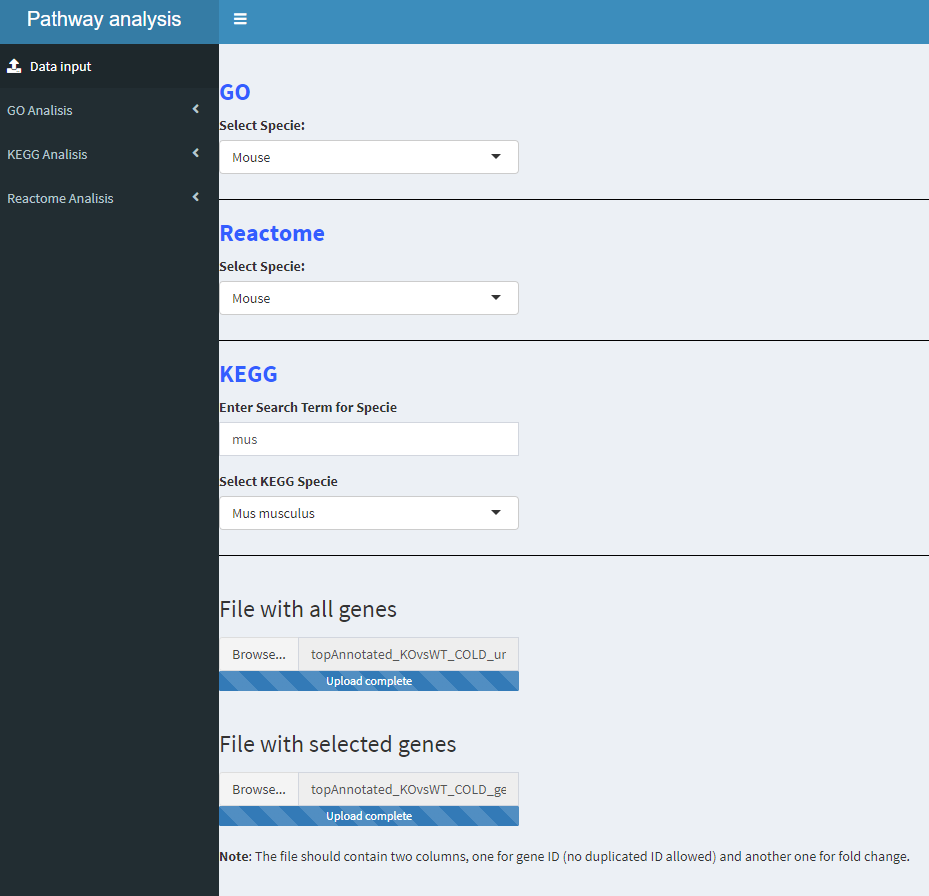
\includegraphics[width=0.6\textwidth]{Estudi1_Fig1_Select_Specie.png} 
\caption{Selecció d'espècie}
\end{figure}

L'output a baix indica que s'ha pujat el total de 5995 gens. Per a l'arxiu dels gens seleccionats l'aplicació diu que s'han pujat 769 gens.

\begin{figure}[H]
\centering
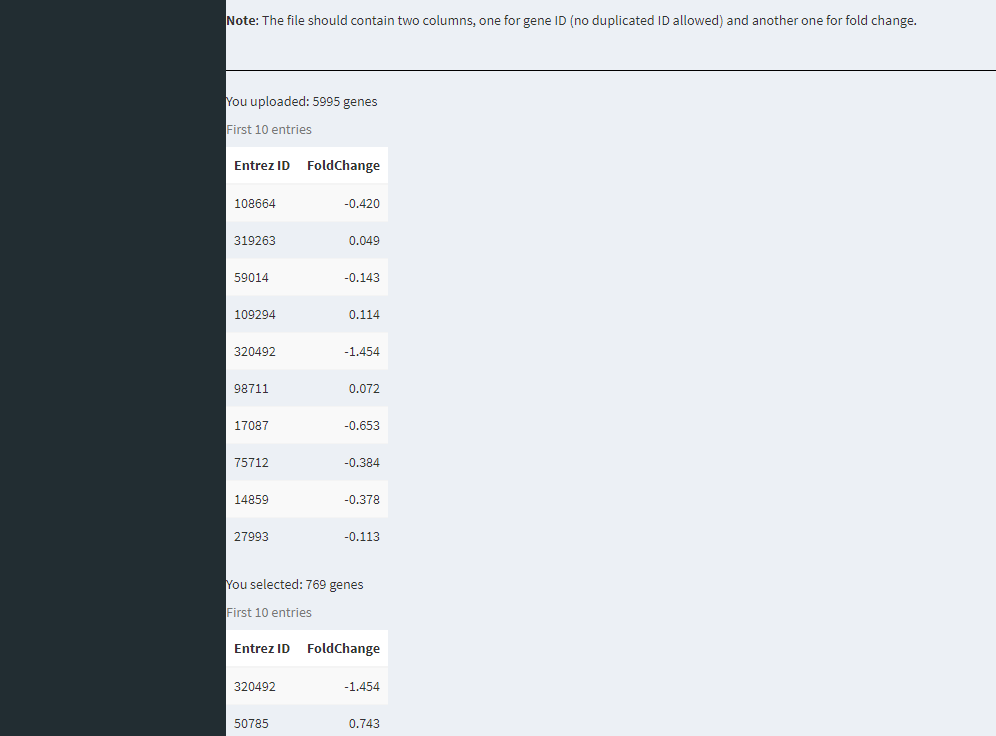
\includegraphics[width=0.6\textwidth]{Estudi1_Fig2_Select_Specie.png} 
\caption{Selecció d'espècie}
\end{figure}


\item Clico en l'apartat \textit{Reactome Analysis}$\rightarrow$\textit{ORA}. Selecciono com a mètode d'ajustament \textit{BH} i el cut-off del valor de P ajustat 0.05. Clico a \textit{Calculate results}

\begin{figure}[H]
\centering
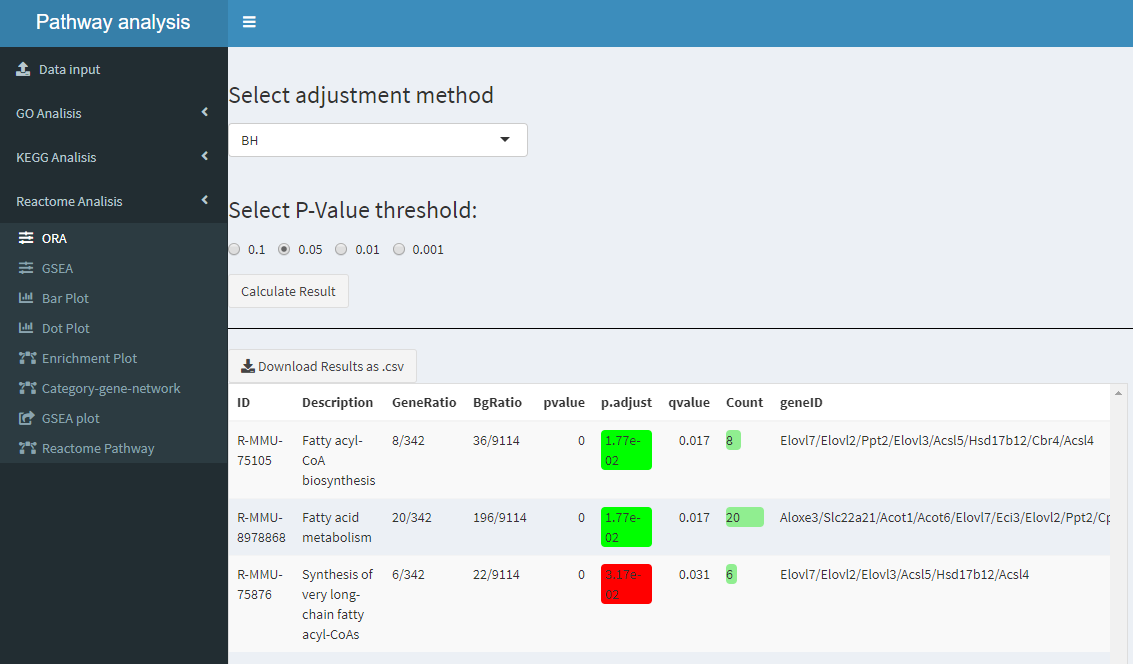
\includegraphics[width=0.6\textwidth]{Estudi1_Fig3_ORA_RA.png} 
\caption{Resultat d'anàlisi ORA de Reactome}
\end{figure}

Observem que els gens mostrats són els mateixos esmentats per Sanz i Pla.

\item Visualització del resultat ORA

\begin{itemize}
\item Selecciono \textit{Reactome Analysis}$\rightarrow$\textit{Bar Plot}

\begin{figure}[H]
\centering
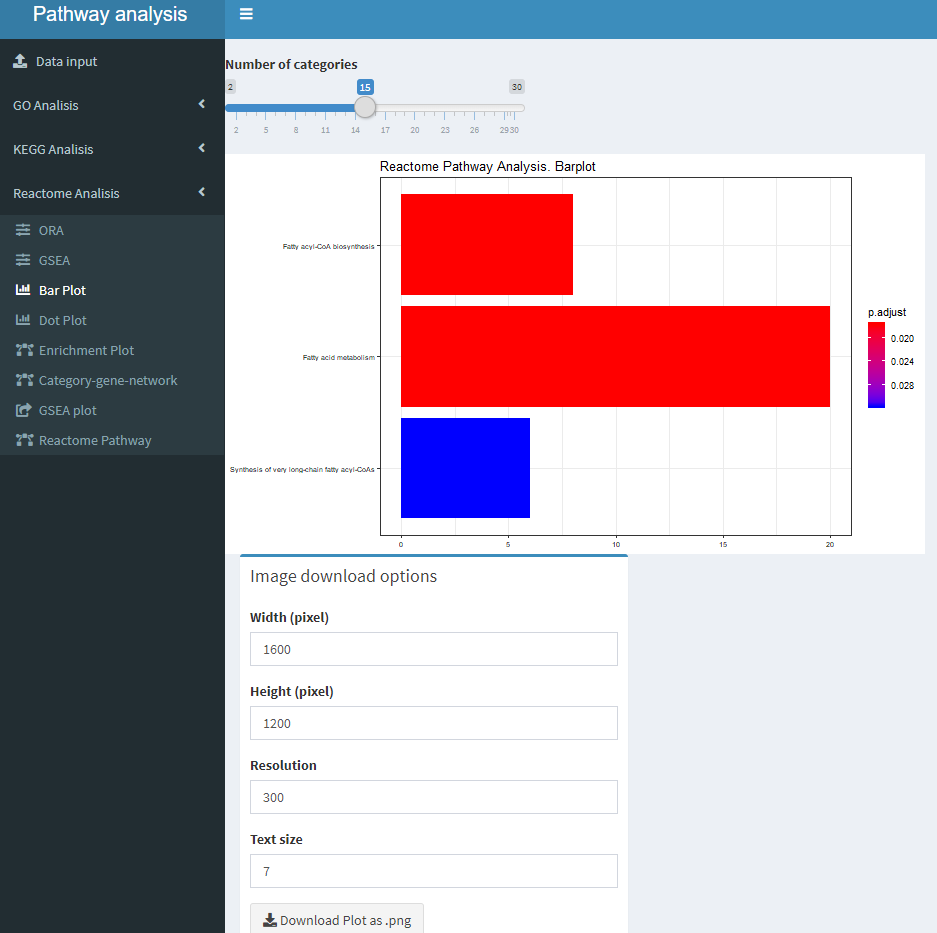
\includegraphics[width=0.6\textwidth]{Estudi1_Fig4_ORA_BP_RA.png} 
\caption{Gràfic de barres}
\end{figure}

\item Selecciono \textit{Reactome Analysis}$\rightarrow$\textit{Dot Plot}

\begin{figure}[H]
\centering
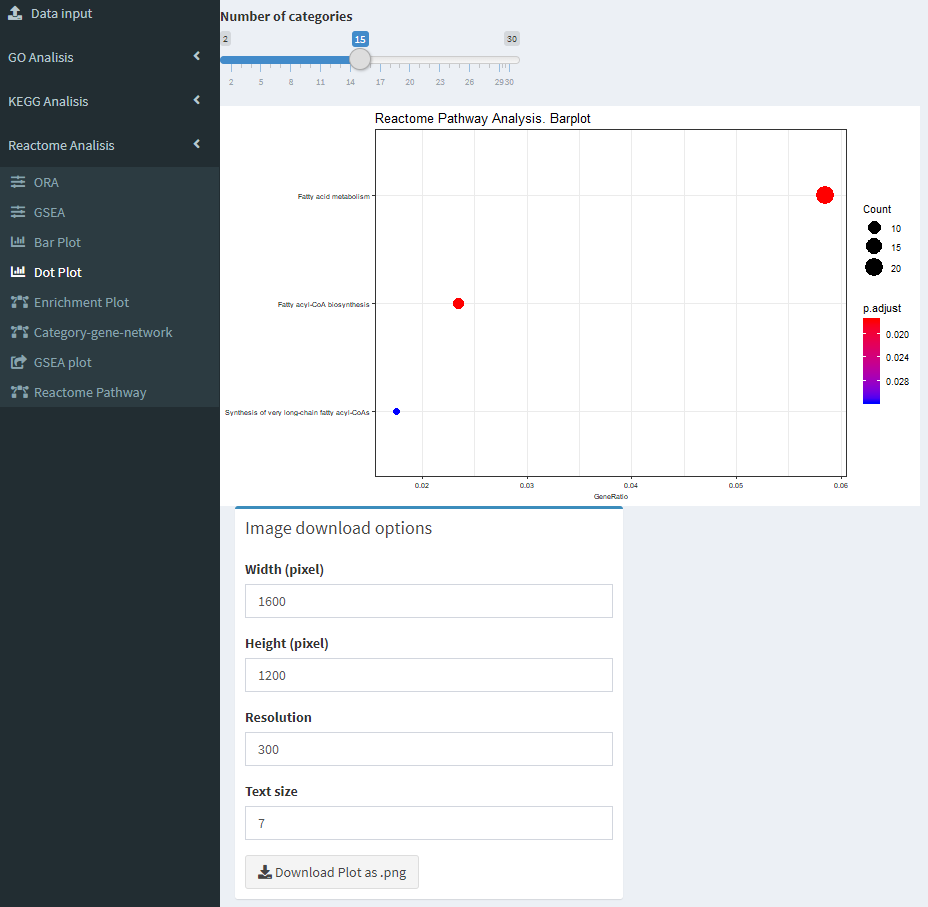
\includegraphics[width=0.6\textwidth]{Estudi1_Fig5_ORA_Dot_RA.png} 
\caption{Gràfic de punts}
\end{figure}

\item Selecciono \textit{Reactome Analysis}$\rightarrow$\textit{Enrichment Map Plot}

\begin{figure}[H]
\centering
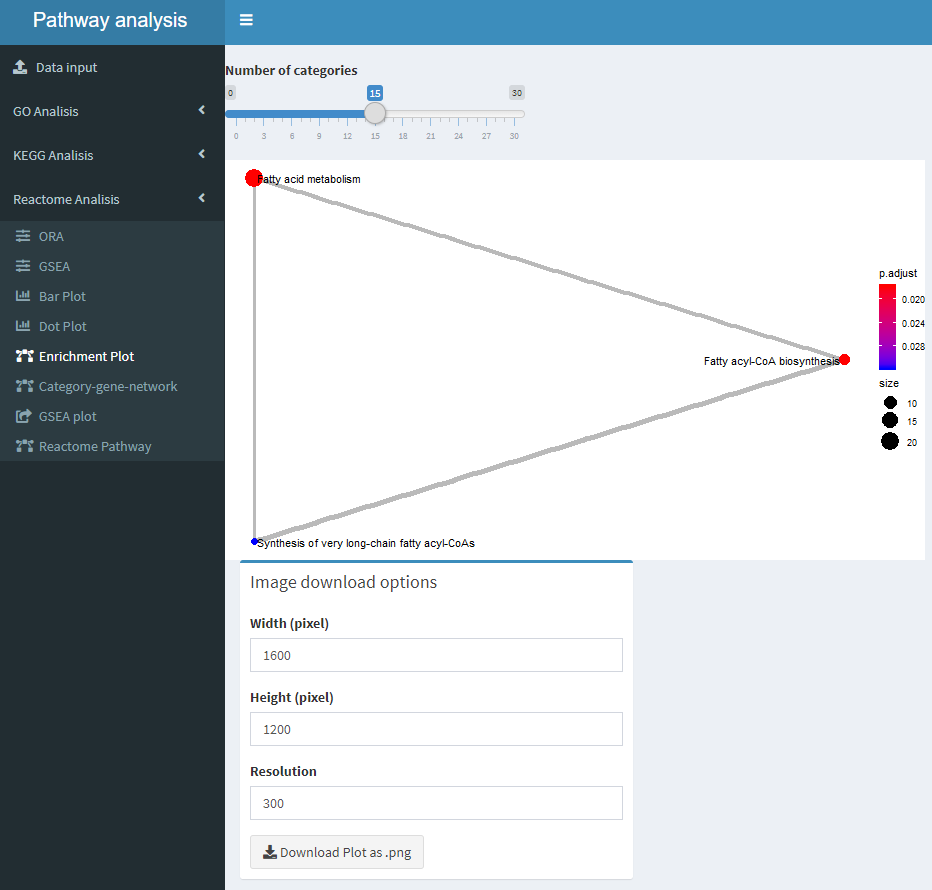
\includegraphics[width=0.6\textwidth]{Estudi1_Fig6_ORA_EP_RA.png} 
\caption{Mapa d'enriquement}
\end{figure}

\item Selecciono \textit{Reactome Analysis}$\rightarrow$\textit{Category Gene Network}
\begin{figure}[H]
\centering
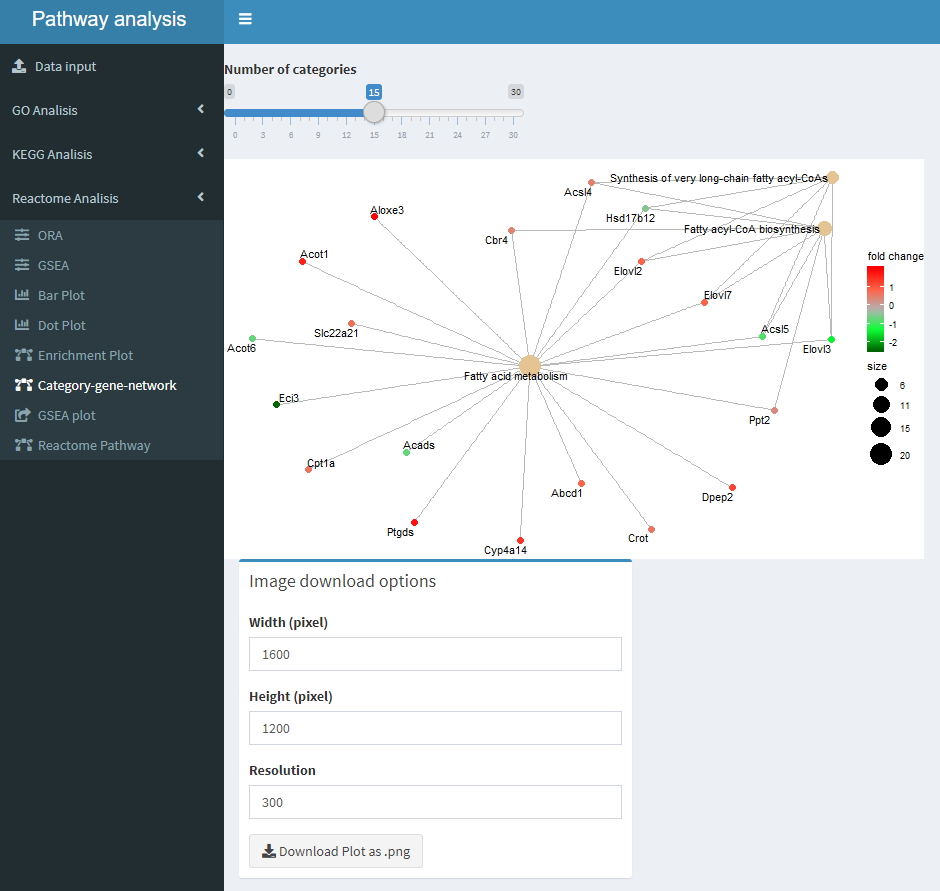
\includegraphics[width=0.6\textwidth]{Estudi1_Fig7_ORA_CP_RA.png} 
\caption{Red de les categories i gens}
\end{figure}

\item Selecciono \textit{Reactome Analysis}$\rightarrow$\textit{Reactome Pathway}
\begin{figure}[H]
\centering
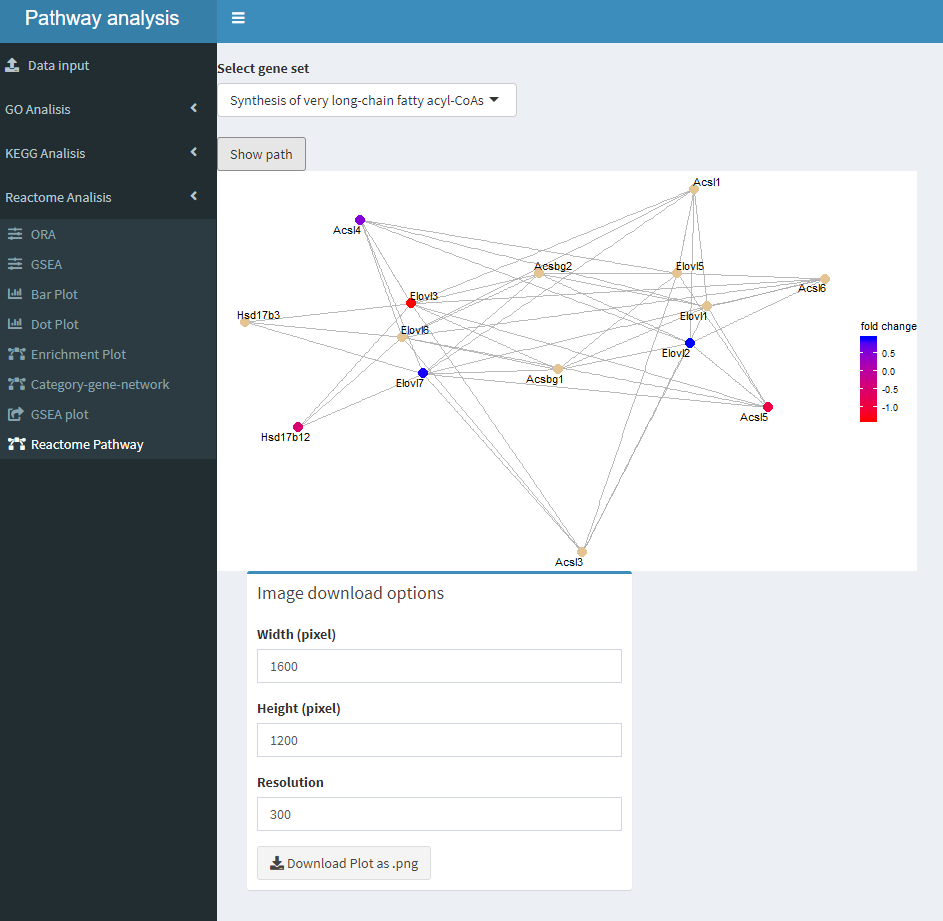
\includegraphics[width=0.6\textwidth]{Estudi1_Fig8_ORA_PP_RA.png} 
\caption{Rutes Reactome}
\end{figure}
\end{itemize}
\end{enumerate}

Addicionalment a l'anàlisi ORA podem fer, mitjançant l'aplicació, l'anàlisi GSEA per les rutes de Reactome. Per fer-ho:

\begin{enumerate}

\item Clico en l'apartat \textit{Reactome Analysis}$\rightarrow$\textit{GSEA}. Selecciono com a mètode d'ajustament \textit{BH} i el cut-off del valor de P ajustat 0.05. Clico a \textit{Calculate results}

Amb el valor de P de 0.05 l'anàlisi no troba cap ruta enriquida.

\item Augmento el Cut-Off del valor de P a 0.1

Amb el Cut-Off més alt l'aplicació retorna un llistat de gens.

\begin{figure}[H]
\centering
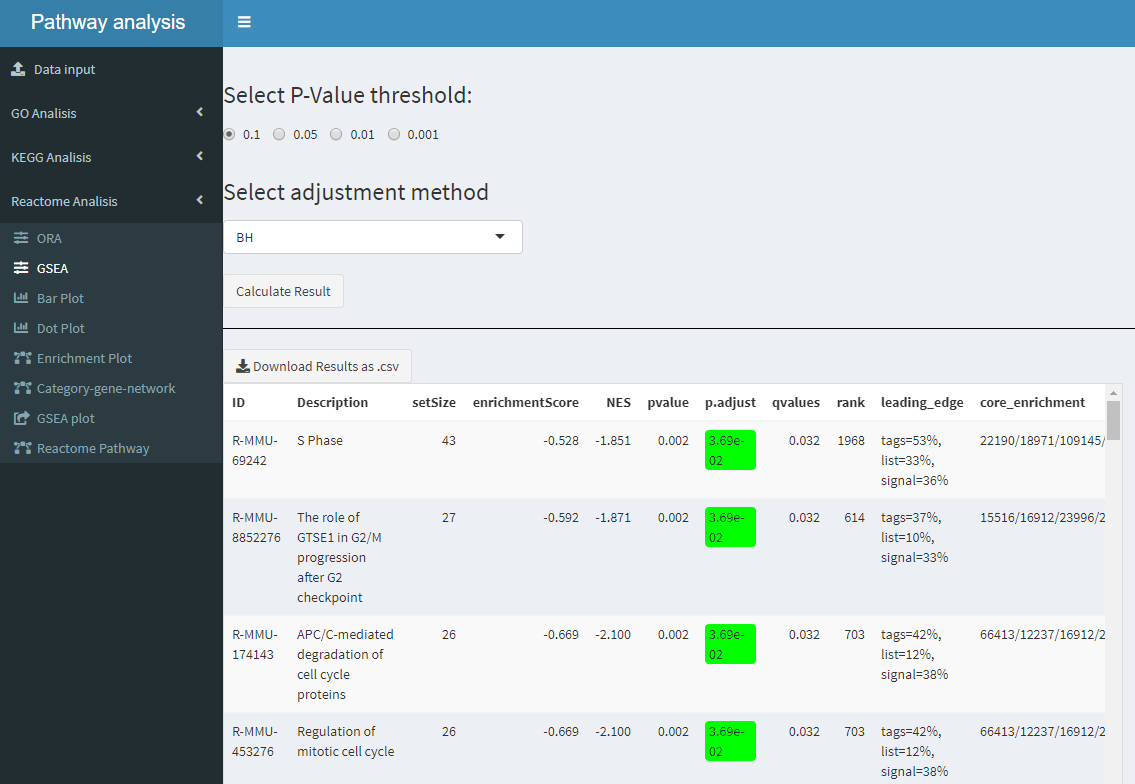
\includegraphics[width=0.6\textwidth]{Estudi1_Fig9_GSEA_RA.png} 
\caption{Anàlisi GSEA}
\end{figure}

\item Per obtenir els gràfics GSEA anem a \textit{Reactome Analysis}$\rightarrow$\textit{GSEA plot}

\begin{figure}[H]
\centering
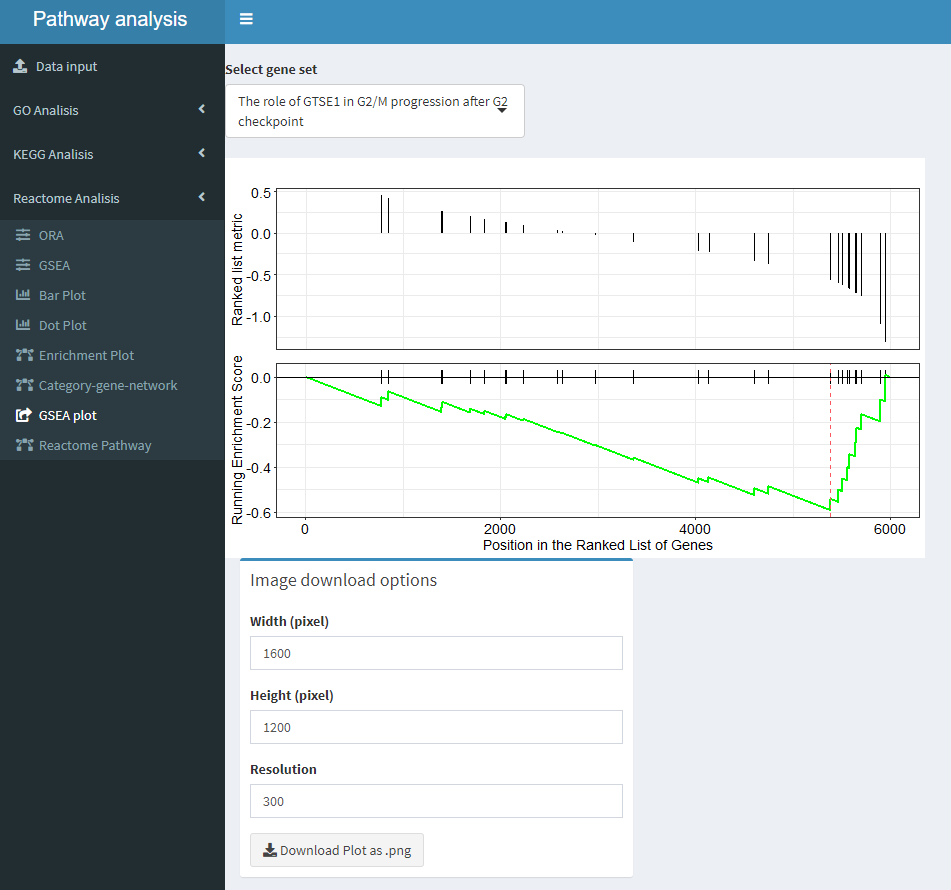
\includegraphics[width=0.6\textwidth]{Estudi1_Fig10_GSEA_RA.png} 
\caption{Gràfic GSEA}
\end{figure}
\end{enumerate}

També podem fer l'anàlisi de KEGG. El resultat de KEGG és similar a l'anàlisi de Reactome. L'aplicació permet però generar les rutes KEGG. Per obtenir-les:

\begin{enumerate}
\item Clico en l'apartat \textit{KEGG Analysis}$\rightarrow$\textit{ORA}. Selecciono com a mètode d'ajustament \textit{BH} i el cut-off del valor de P ajustat 0.05. Clico a \textit{Calculate results}
\begin{figure}[H]
\centering
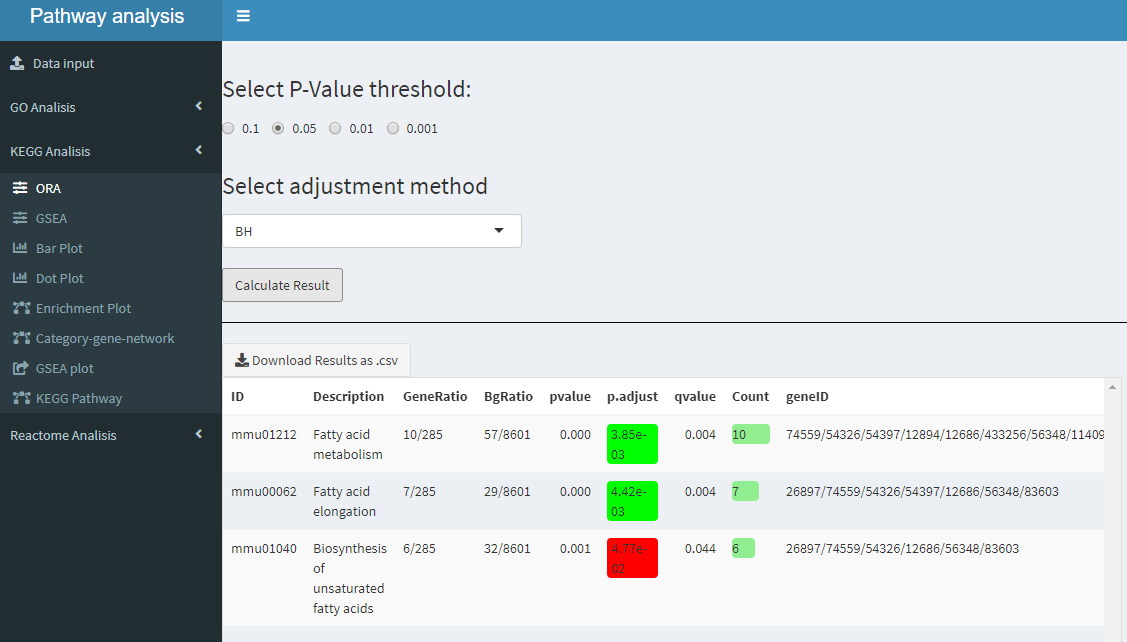
\includegraphics[width=0.6\textwidth]{Estudi1_Fig11_ORA_KEGG.png} 
\caption{Anàlisi ORA de KEGG}
\end{figure}

\item Anem a \textit{KEGG}$\rightarrow$\textit{KEGG Pathway}
\begin{figure}[H]
\centering
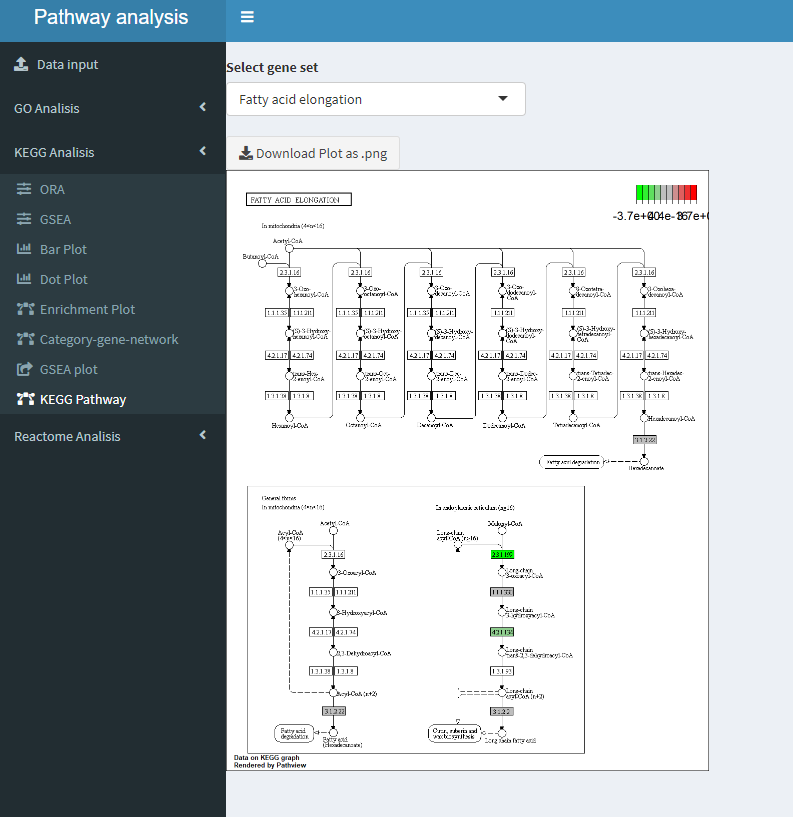
\includegraphics[width=0.6\textwidth]{Estudi1_Fig12_KEGG_Pathway.png} 
\caption{Gràfic de les rutes KEGG}
\end{figure}
\end{enumerate}

L'anàlisi GO no retorna cap terme GO amb el nivell de significació de 0.05. Pujant el nivell de significació fins 0.1 retorna un llistat dels termes enriquits per als components cel·lulars.

Clico en l'apartat \textit{GO Analysis}$\rightarrow$\textit{ORA}. Selecciono com a mètode d'ajustament \textit{BH} i el cut-off del valor de P ajustat 0.1. Selecciono també \textit{CC}. Clico a \textit{Calculate results}
\begin{figure}[H]
\centering
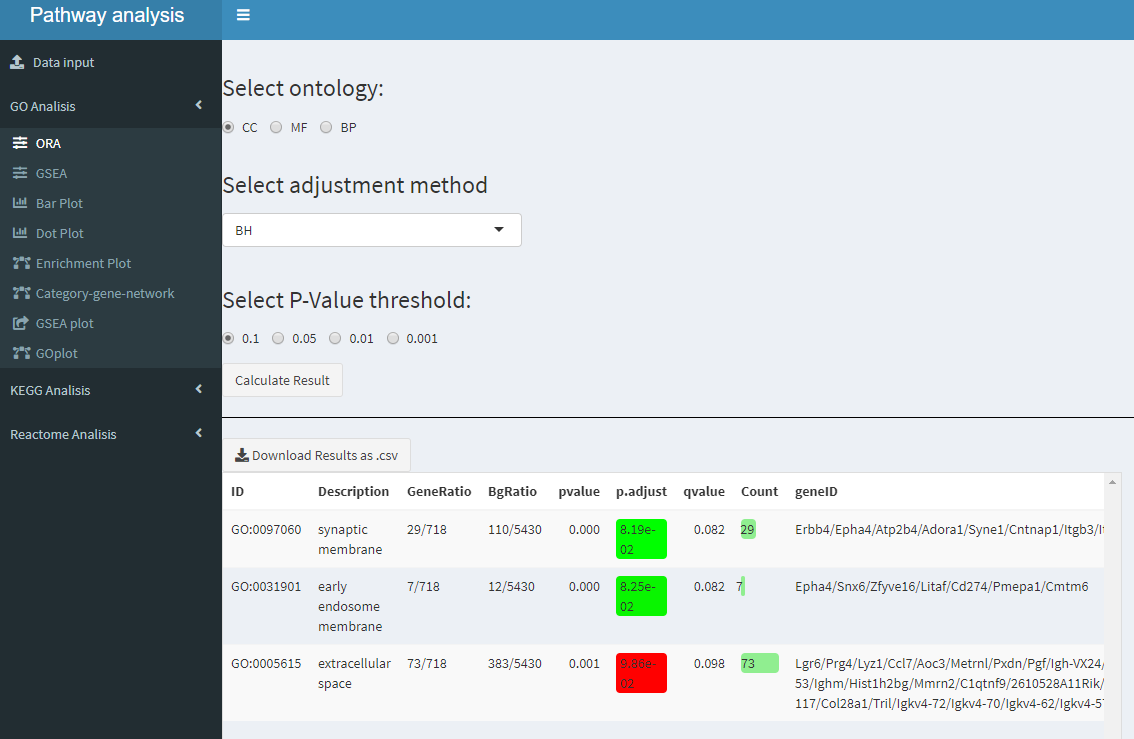
\includegraphics[width=0.6\textwidth]{Estudi1_Fig13_GO.png} 
\caption{L'anàlisi ORA de GO}
\end{figure}

\section{Discussió}

\section*{Biblilografia}
\addcontentsline{toc}{section}{Biblilografia}
\renewcommand{\section}[2]{}%
%\renewcommand{\chapter}[2]{}% for other classes
\bibliography{references}
\bibliographystyle{apalike}


\end{document}



